%%%%%%%%%%%%%%%%%%%%%%%%%%%%%%%%%%%%%%%%%%%%%%%%%%%%%%%%%%%%%%%%%%% 
%                                                                 %
%                            CHAPTER                              %
%                                                                 %
%%%%%%%%%%%%%%%%%%%%%%%%%%%%%%%%%%%%%%%%%%%%%%%%%%%%%%%%%%%%%%%%%%% 
 
\chapter{Implementation}
\label{chap:impl}

The implementation consists of three main parts. First the camera setup will be discussed which will be used to create the datasets in section \ref{sec:impl:dataset}. The images from the dataset will later be processed using convolutional neural networks which will be covered in section \ref{sec:impl:visionalgorithms}.

\section{Camera setup}
\label{sec:impl:camerasetup}
As stated in the previous chapter, a new dataset must be created with images of worn tool inserts. For the creation of the dataset a setup is created that consists of three different parts:
\begin{enumerate}
\item A tool holder which will provide the same position of the tool insert for every picture.
\item A mount for the microscopic camera which is stable and easy to finetune.
\item Some lighting solution that provides the right angle of light to the tool insert and reflects into the camera.
\end{enumerate}

These parts will be handled in the following sections starting with the design of a tool holder 
	\subsection{Design of a tool holder}
	The tool holder will be the most important part of the setup since this part will be holding the tool insert where every imperfection will be seen on the output images. The requirements for this holder are:
	\begin{itemize}
	\item The inserts should be easy to remove and to replace.
	\item The holder may not block the view from the camera to the insert.
\end{itemize}	
	
	Since this is a design process there are a few iterations made on these tool holders. The most important are observed in the succeeding sections.
	
	
	\subsubsection{First tool holder}
	\label{sec:impl:camerasetup:firsttoolholder}
	All tool holder prototypes where 3D printed. A first holder was made to check how the lighting would be transferred to the camera. This was put in a simple setup with a desk lamp and a socket which kept the insert at an angle of 40\textdegree. The socket can be found on Figure \ref{fig:impl:setup:fth}. This showed potential in the current setup as seen in Figure \ref{fig:setup:desklamp:whitebg}. The tool wear is nicely indicated with the reflections of the light. 
	
	\begin{figure}[hbtp]
	\centering
	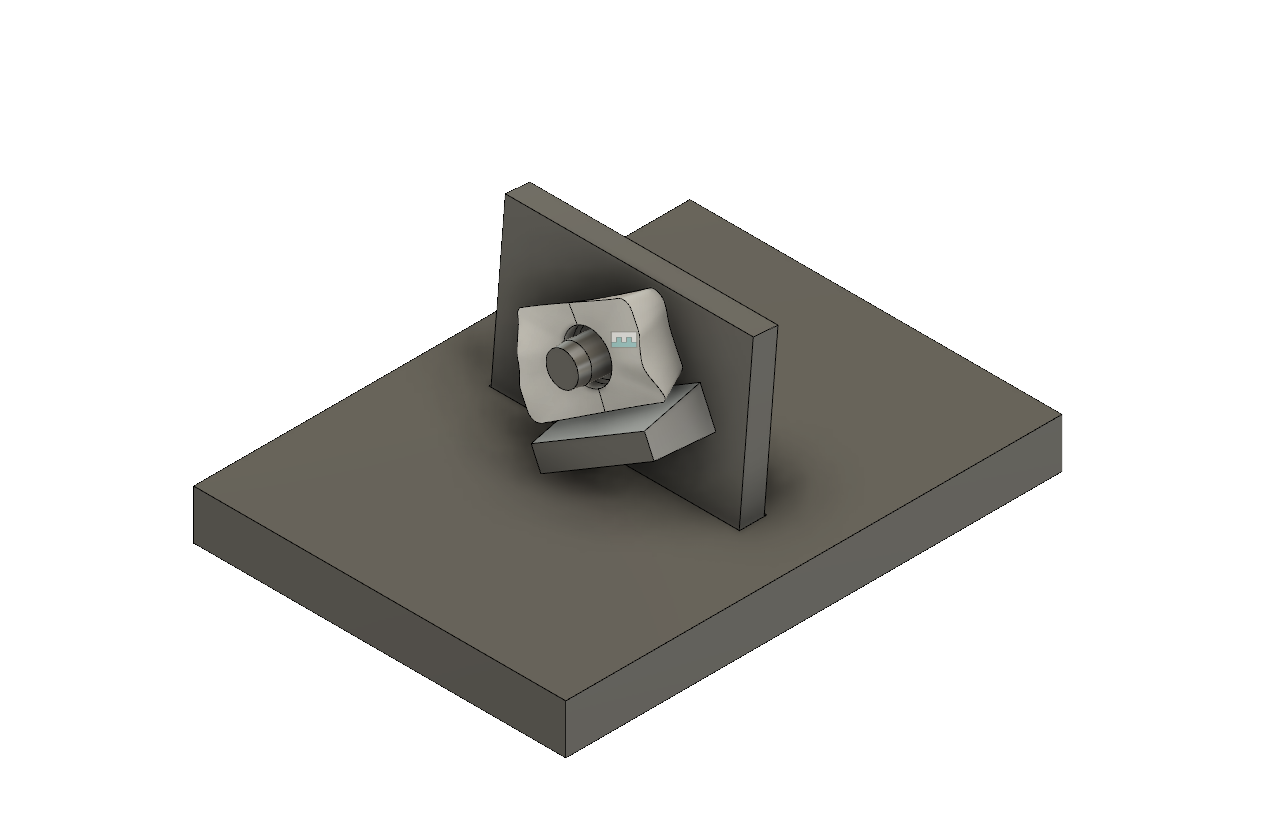
\includegraphics[scale=0.2]{fig/Camera_setup/Tool_Holder/simpeleHouder_attaached.png}
	\caption{First design of a tool holder oriented at an angle of 40\textdegree to the camera.}
	\label{fig:impl:setup:fth}
	\end{figure}
	
	
	\begin{figure}[hbtp]
		\centering
		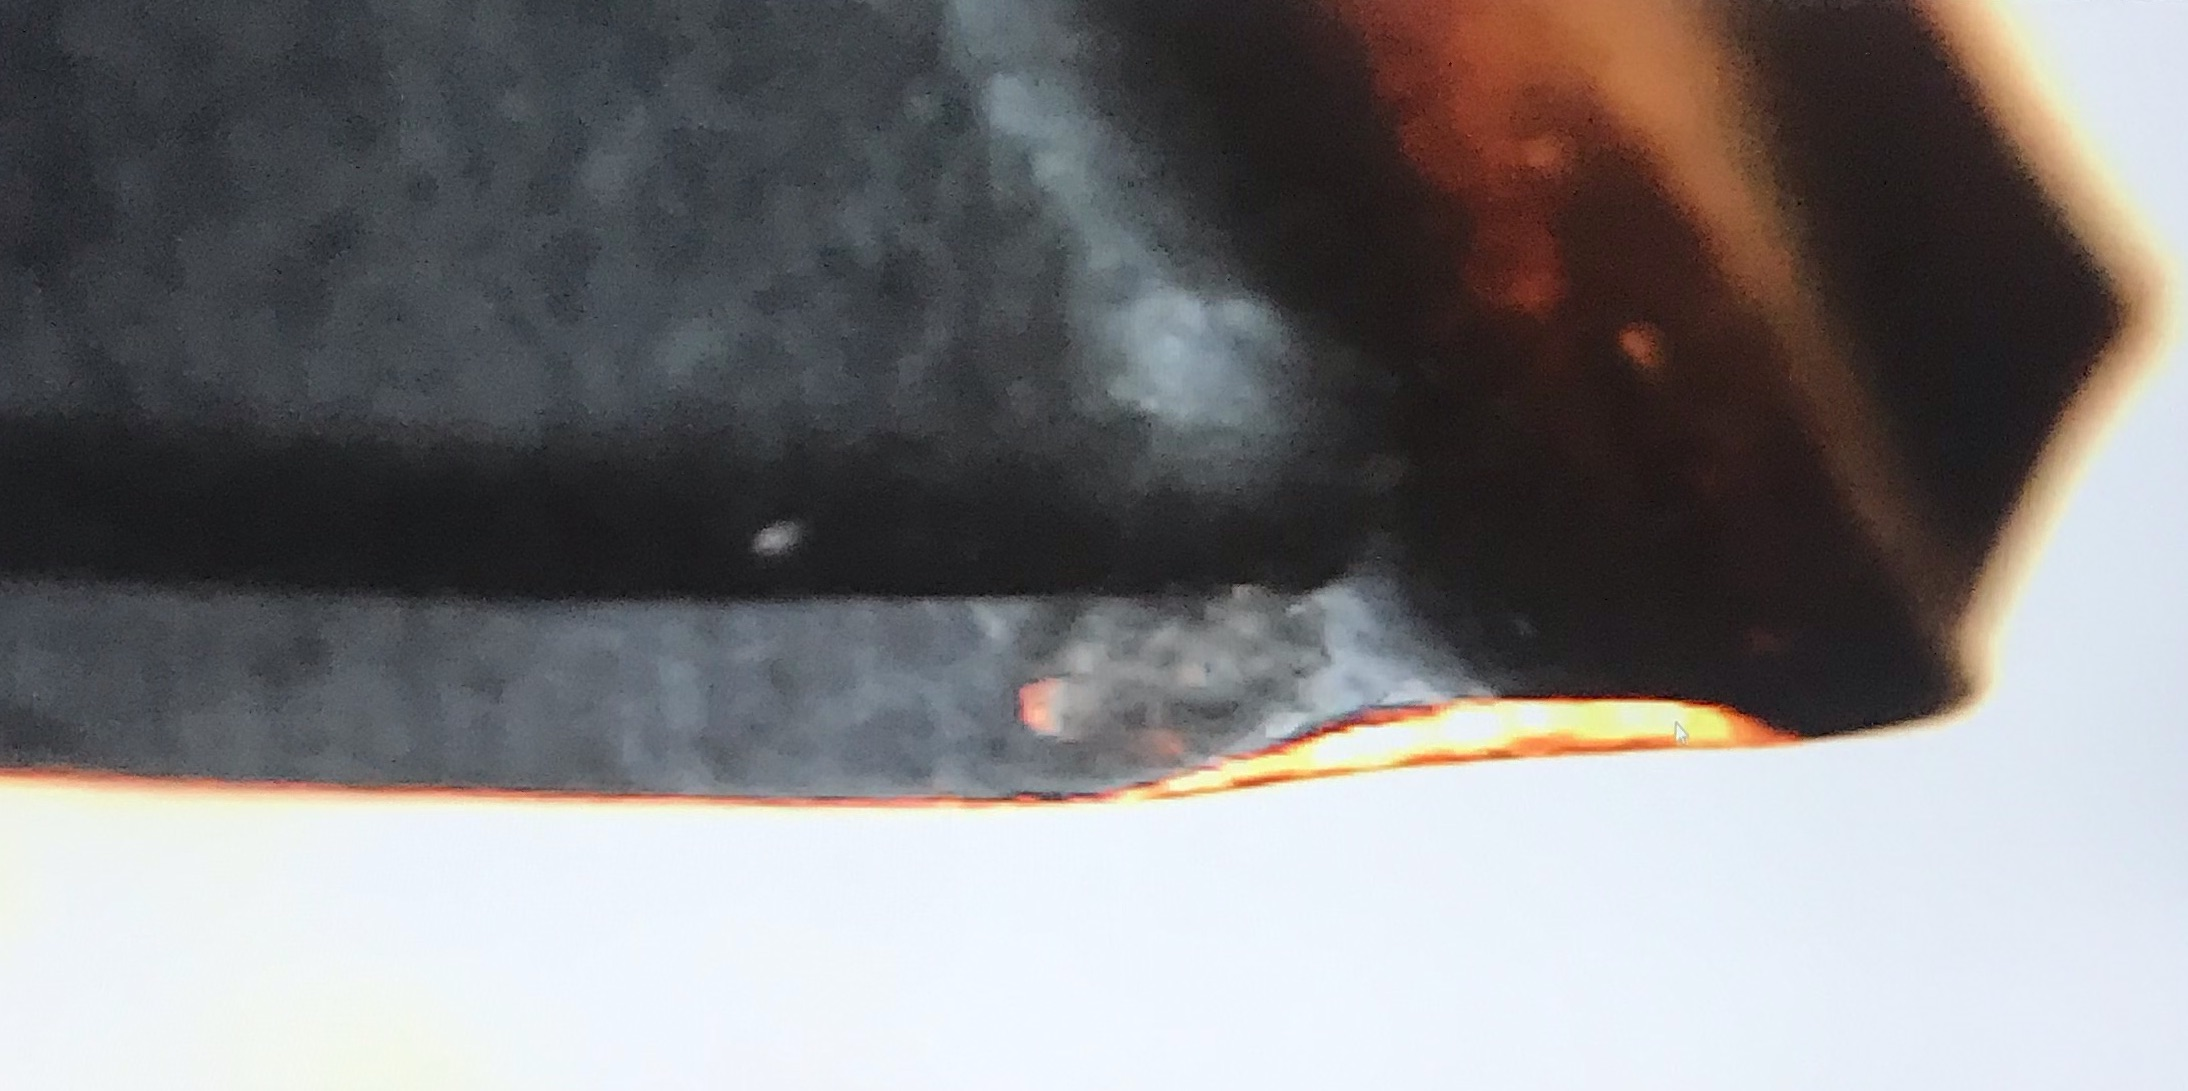
\includegraphics[scale=0.2]{fig/Camera_setup/Light/Desk_Lamp_Test/desk_lamp_setup_whitebg.jpeg}
		\caption{Desk lamp setup without shadowing the background.}
		\label{fig:setup:desklamp:whitebg}
	\end{figure}
	

	\subsubsection{Wheel holder}
	\ref{sec:impl:camerasetup:wheelholder}
	The previous first tool holder was good for taking a sample picture of an insert but isn't scalable to take pictures of a few hundreds of inserts.
	To be able to quickly create a lot of photos in a consistant manner, a wheel is designed to mount 20 inserts at once. With the use of a stepper motor, a fixed camera and lighting setup, the process of taking images is automated for every 20 tools. The holder is 3D printed so a few wheels can be made to be able to swap the wheels with new inserts for an efficient dataset creation.
	
		The first design of this wheel holder can be seen in Figure \ref{fig:setup:wheelholder1:inserts}. 
		The whole wheel is printed in one piece. The inserts are kept in place with brackets that go over the cutting edge of the insert. This didn't seem ideal since the sharp edges of the insert would cut in the bracket what made it very hard to remove the tools which didn't comply with the easy removal constraint. 
		
		\begin{figure}[hbtp]
		\centering
		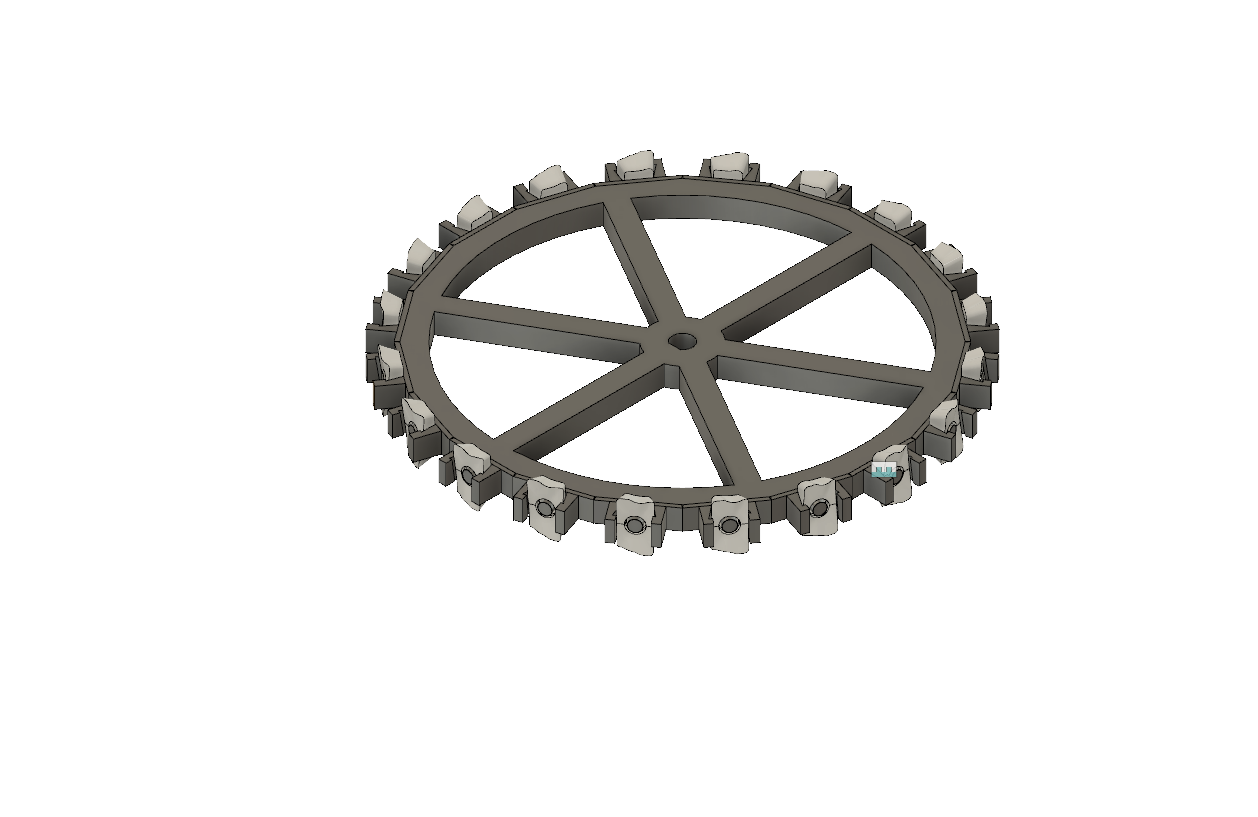
\includegraphics[width=0.5\textwidth]{fig/Camera_setup/Tool_Holder/Wheel_Holder/first_wheel_holder/radhouderV1_model_inserts.png}
		\caption{First design of wheel holder with inserts mounted in place.}
		\label{fig:setup:wheelholder1:inserts}
		\end{figure}
		
		For this reason a second wheel was designed which was a little more flexible and made the process of inserting and replacing tools a lot easier by providing a clip which was printed and added to the wheel separately. Figure \ref{fig:setup:wheelholder2:inserts} shows the full assembly of this second wheel holder. 
		
		
		\begin{figure}[hbtp]
		\centering
		\begin{subfigure}{0.49\textwidth}
			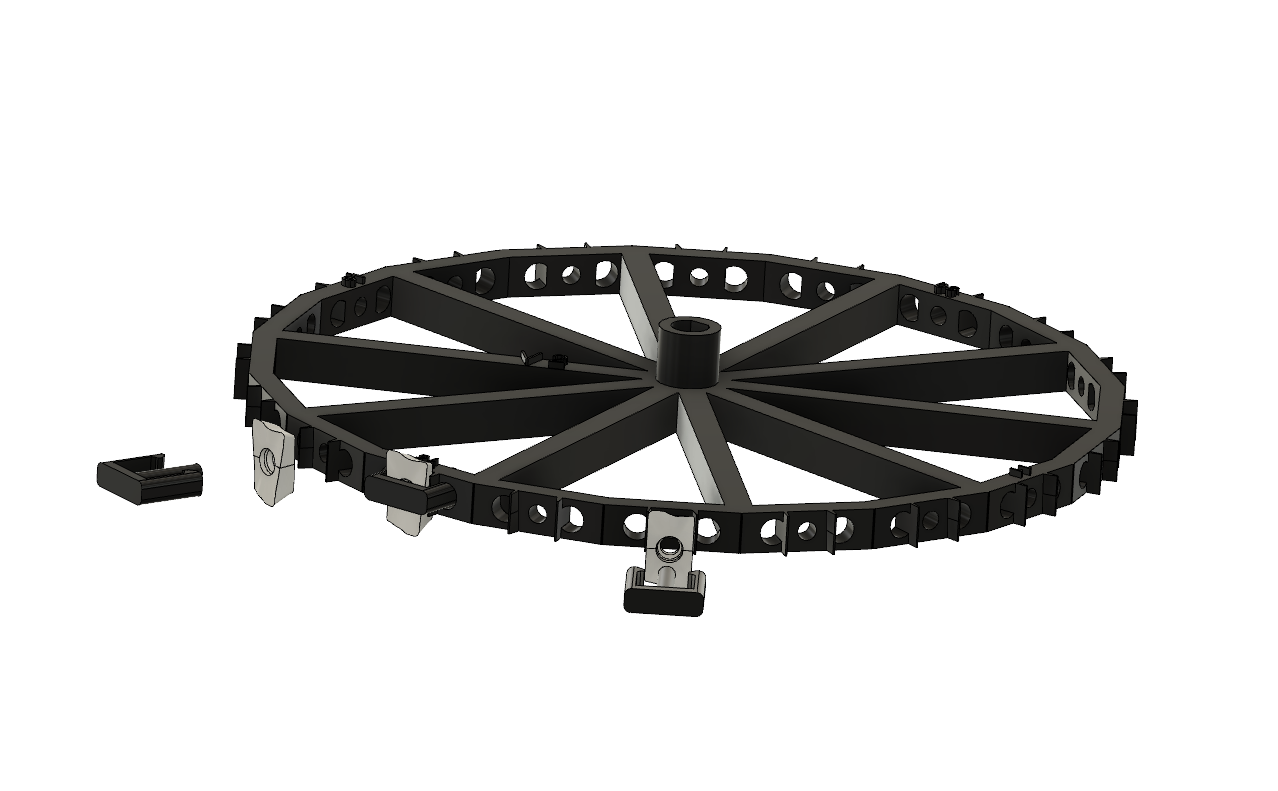
\includegraphics[width=\linewidth]{fig/Camera_setup/Tool_Holder/Wheel_Holder/Second_Wheel_Holder/radhouder_v2_assembly v3 extra insert.png}
			\caption{Illustration of second wheel holder.}
			\label{fig:setup:wheelholder2:inserts}
		\end{subfigure}
		\hspace*{\fill}
		\begin{subfigure}{0.49\textwidth}
			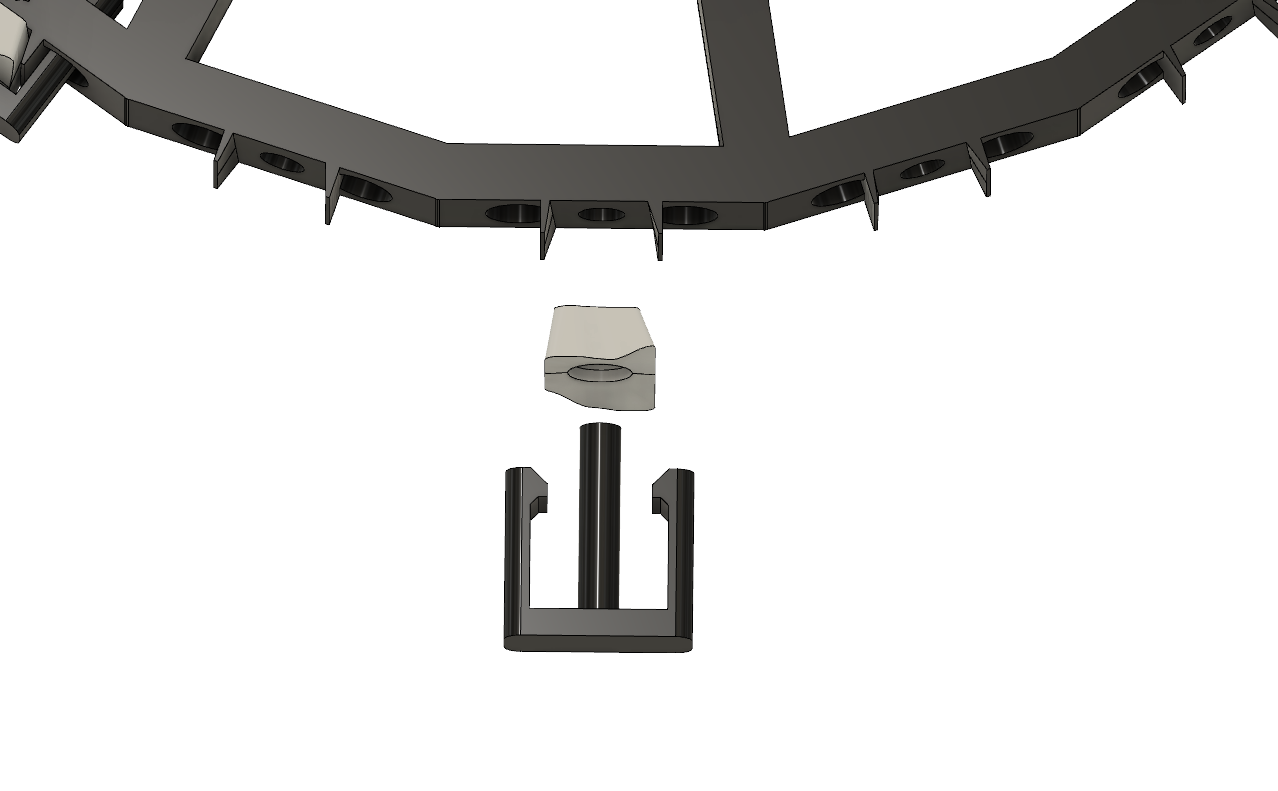
\includegraphics[width=\linewidth]{fig/Camera_setup/Tool_Holder/Wheel_Holder/Second_Wheel_Holder/radhouder_v2_assembly v3 top view insert.png}
			\caption{Zoomed illustration with clip and insert.}
			\label{fig:setup:wheelholder2:topinserts}
		\end{subfigure}
		\caption{Overview of second wheel holder}
		\end{figure}
		
		In the wheel there are holes in which the clips fit. The center hole is as big as the hole in the inserts. This keeps the insert from moving when the clip is on. The slads between the holes are made to fit the insert perfectly so this doesn't rotate around the axis of the clip. On the clip there is an extra long middle tube that makes it easier to push the clip with the insert out of the wheel. This can all be seen in a close up on Figure \ref{fig:setup:wheelholder2:topinserts}.
		
	\subsection{Design of a camera mount}
	\label{sec:impl:camerasetup:cameramount} 
	In this section the camera mount will be discussed along the design process of the setup.
		The camera mount provided by the factory was not up to the task of taking consistent pictures and controlling the camera position precisely so a new camera mount was designed. For this task some 20mm by 20mm aluminium profiles where used as a base for the stand. On that stand an assembly of 3D printed parts where mounted to be able to rotate the camera around two different axis as seen on the close up on Figure \ref{fig:impl:cs:cameramount:zoom}. 
		
		A render of the full assembly of this new camera mount can be found in Figure \ref{fig:impl:cs:cameramount:full}.
		
		\begin{figure}[hbtp]
		\centering
		\begin{subfigure}{0.49\textwidth}
			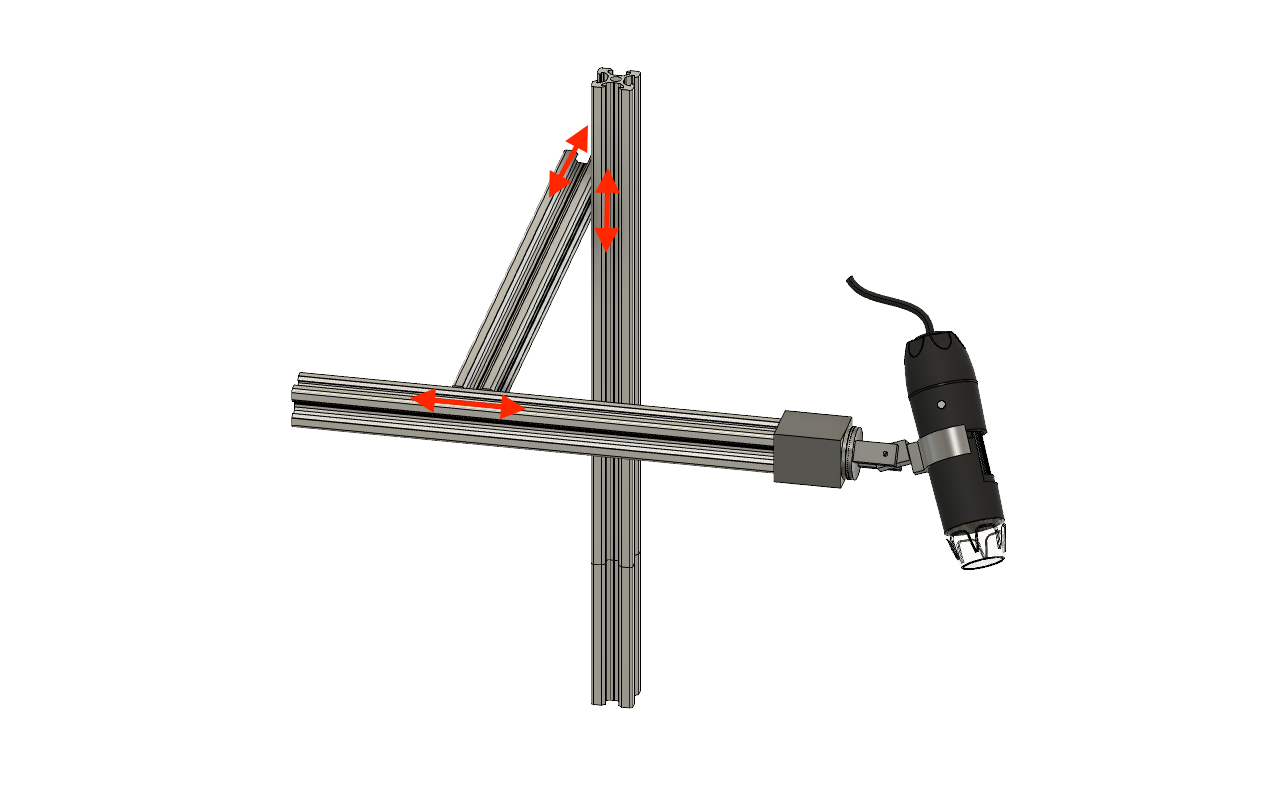
\includegraphics[width=\linewidth]{fig/Camera_setup/camera_mount/second_camera_mount/camera mount v9 back top.png}
			\caption{A render of the camera mount with the given movement options.}
			\label{fig:impl:cs:cameramount:full}
		\end{subfigure}
		\hspace*{\fill}
		\begin{subfigure}{0.49\textwidth}
			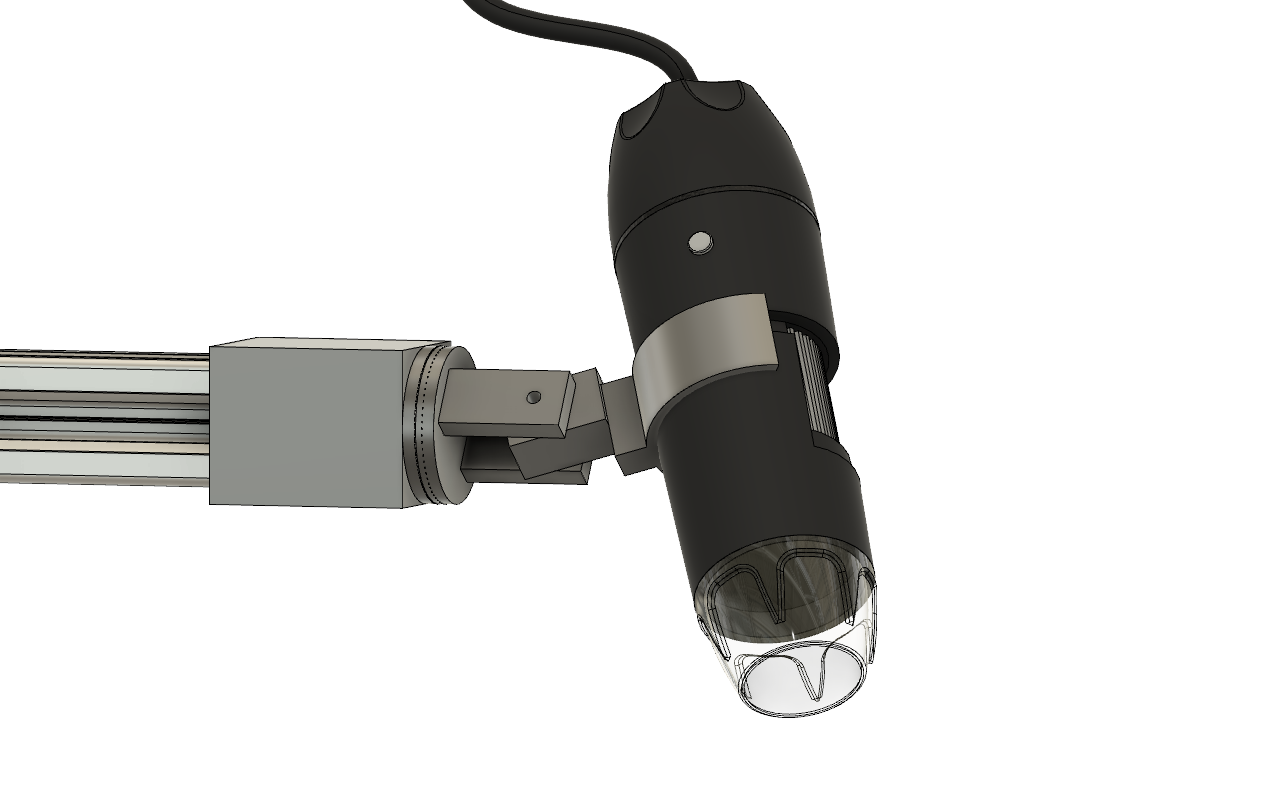
\includegraphics[width=\linewidth]{fig/Camera_setup/camera_mount/second_camera_mount/camera mount v9 zoom camera.png}
			\caption{Close up to the rotation and hinge for the camera.}
			\label{fig:impl:cs:cameramount:zoom}
		\end{subfigure}
		\caption{Overview of the camera mount system.}
		\end{figure}
		
		
	\subsection{Light configuration}
	In order to test different lighting options there must be a simple to configure lighting solution. This should be configurable in both color and light direction to create a maximum reflection of the wear area into the camera lens. This is achieved with single LED adressable LED strips.
	
	Multiple different light sources where tested as listed underneath. Some worth noticing are declared after.

		\begin{enumerate}
			\item Warm white LED desk Lamp
			\item Long hard white LED strips 
			\item single LED adressable RGB LED strip
			\item Multiple single LED adressable RGB strips
			\item USB microscope camera light
		\end{enumerate}
		
		\subsubsection{Desk Lamp Test}

			As an initial setup to test the camera and be able to see the effects of lighting on the image this setup was created and a desk lamp was used for the lighting as seen in Figure \ref{fig:setup:desklamp}. On this Figure we can also see the initial tool holder from section \ref{sec:impl:camerasetup:firsttoolholder}.

			\begin{figure}[hbtp]
				\centering
				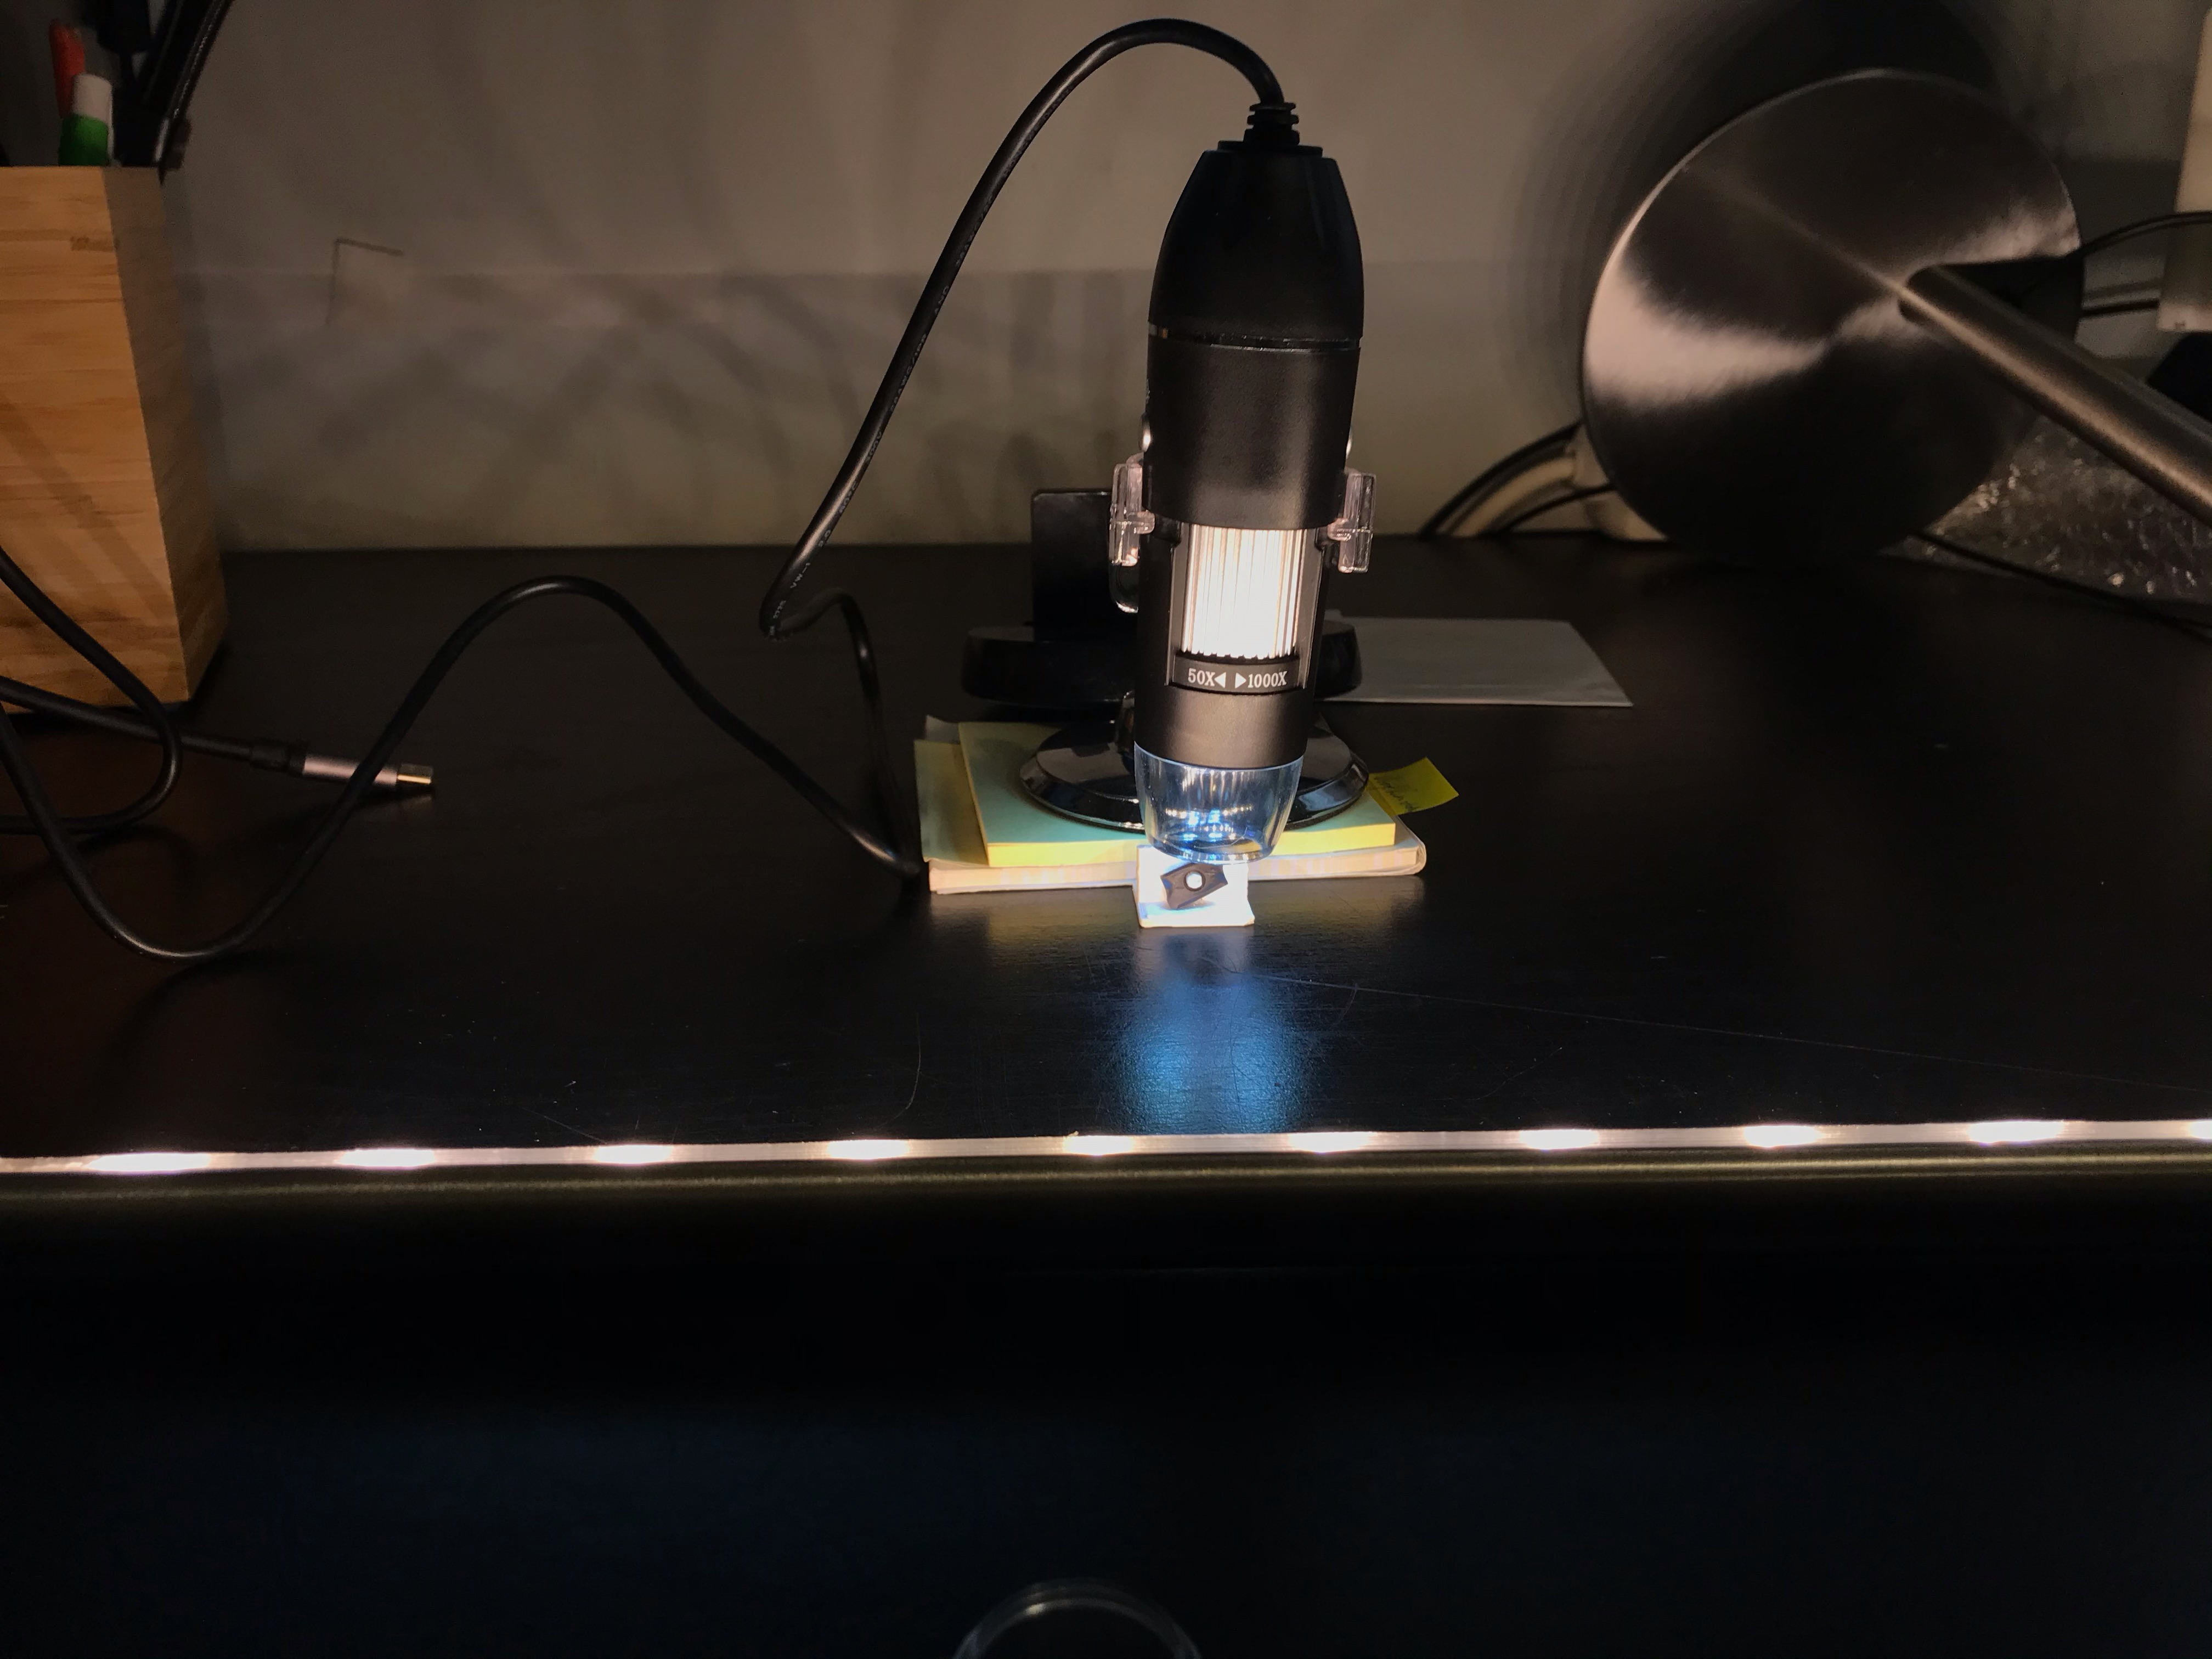
\includegraphics[width=0.55\textwidth, keepaspectratio=true]{./fig/Camera_setup/Light/Desk_Lamp_Test/eerste_setup_andere_richting.jpeg}
				\caption{Desk lamp setup for initial testing.}
				\label{fig:setup:desklamp}
			\end{figure}

			This setup used the top light of the camera which was good to lighten a whole area to adjust the camera. The worn places where more visible without that top lighting. The desk lamp added to much brightness and didn't leave enough room for adjusting different settings. For this reason other lighting options where explored.

From this setup it can also be seen that the lighting on the background is important. Figure \ref{fig:setup:desklamp:whitebg} shows a picture of the tool with desk lamp lighting without blocking the light from the background. Here we can see that there is a bright white background behind the tool. 

The result of this is shown in Figure \ref{fig:setup:desklamp:blackbg} where the light is blocked off of the rest of the tool and only the errornous part is lightened. This would be a good start for creating a dataset.

\begin{figure}[hbtp]
\centering
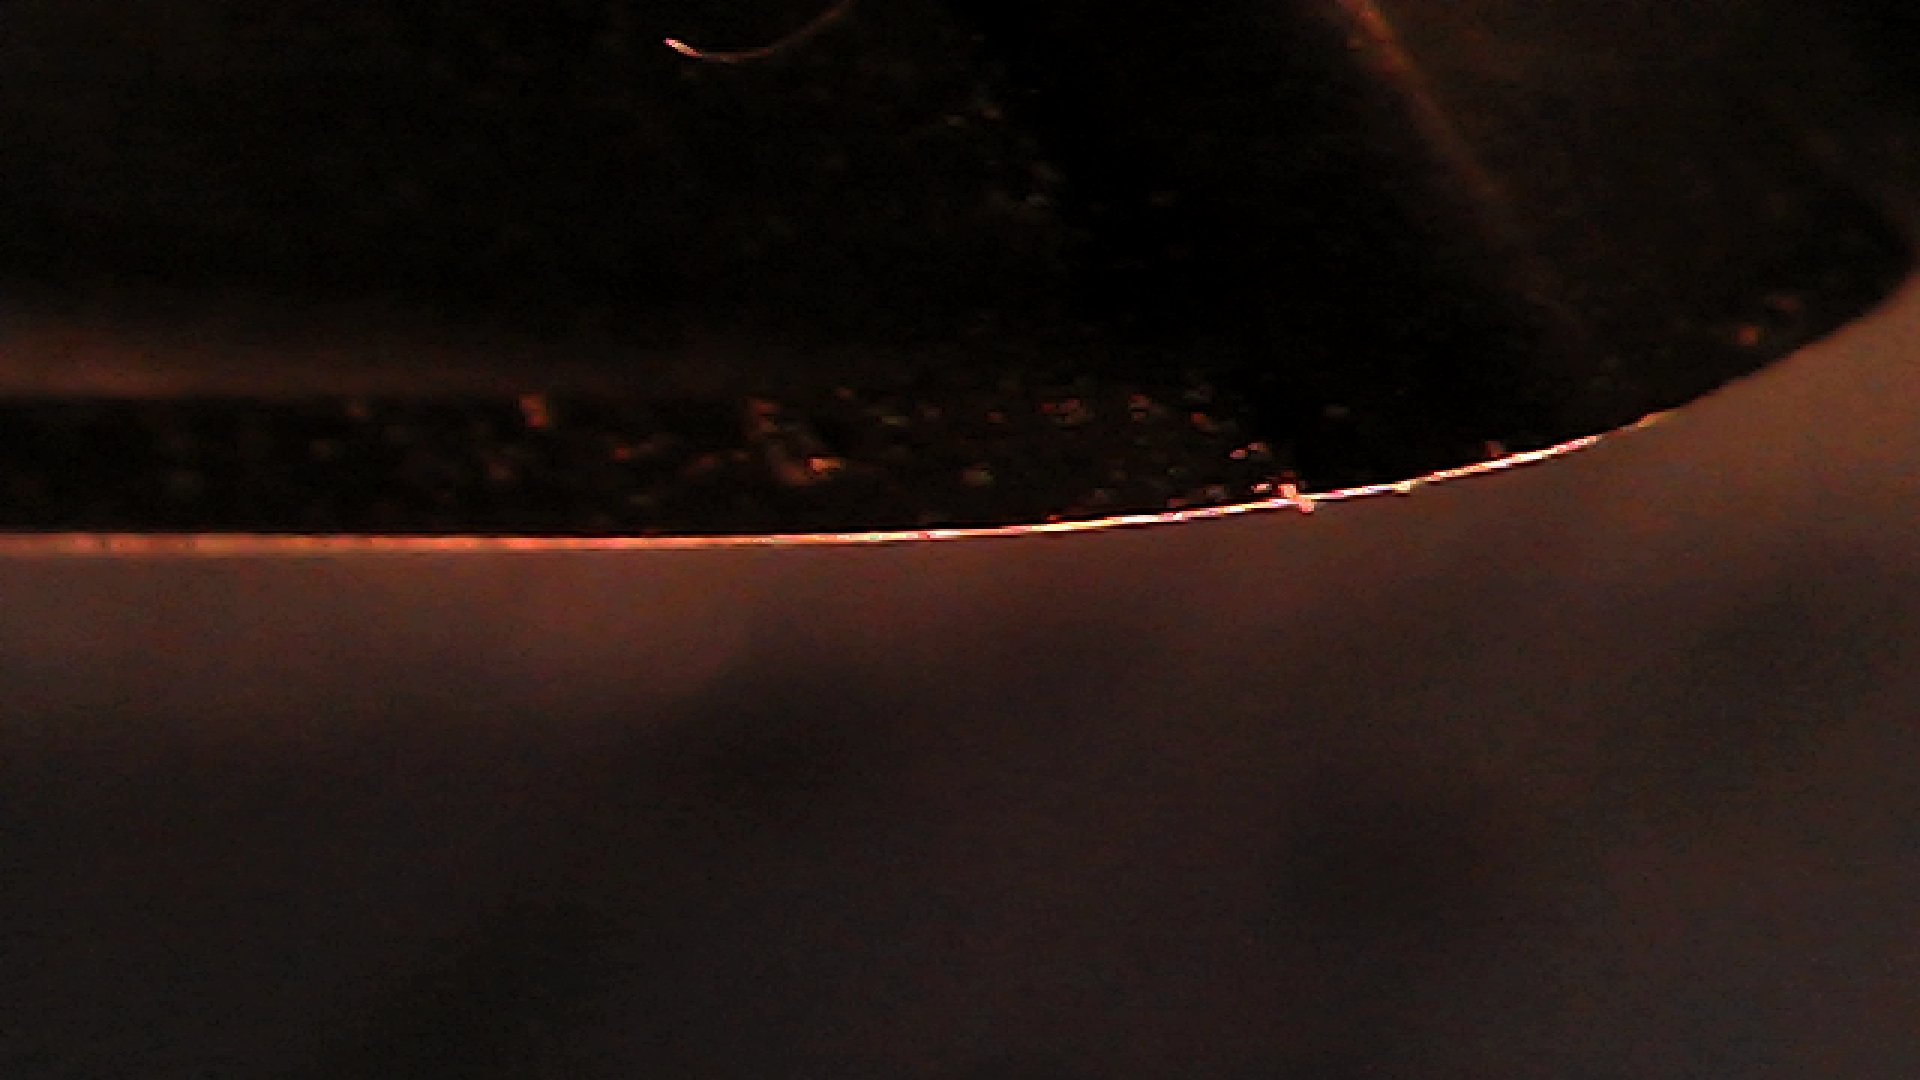
\includegraphics[width=4.166667in, keepaspectratio=true]{./fig/Camera_setup/Light/Desk_Lamp_Test/eerste-opstelling_donkere_achtergrond2.jpg}
\caption{Desk lamp setup with shadowing the background.}
\label{fig:setup:desklamp:blackbg}
\end{figure}

The color of the desk light set a good gradient of bad vs good sets. White areas are worn very hard while orange is not worn that hard. By tilting the lamp in a horizontal way, all the areas where lighted. 

		\subsubsection{White Led Strips}

		A second lighting condition created for this setup uses 3 the similar LED strips controllable with a micro controller. 
		For the purpose of this test a small electric circuit is created to control these strips since they use more power than the raspberry pi can deliver \citep{rpi}. An overview of this test circuit can be found in Figure \ref{fig:setup:whiteled:circuit}. A potentiometer was used to control the voltage over the LED strip in order to control the brightness. 

		\begin{figure}[hbtp]
			\centering
			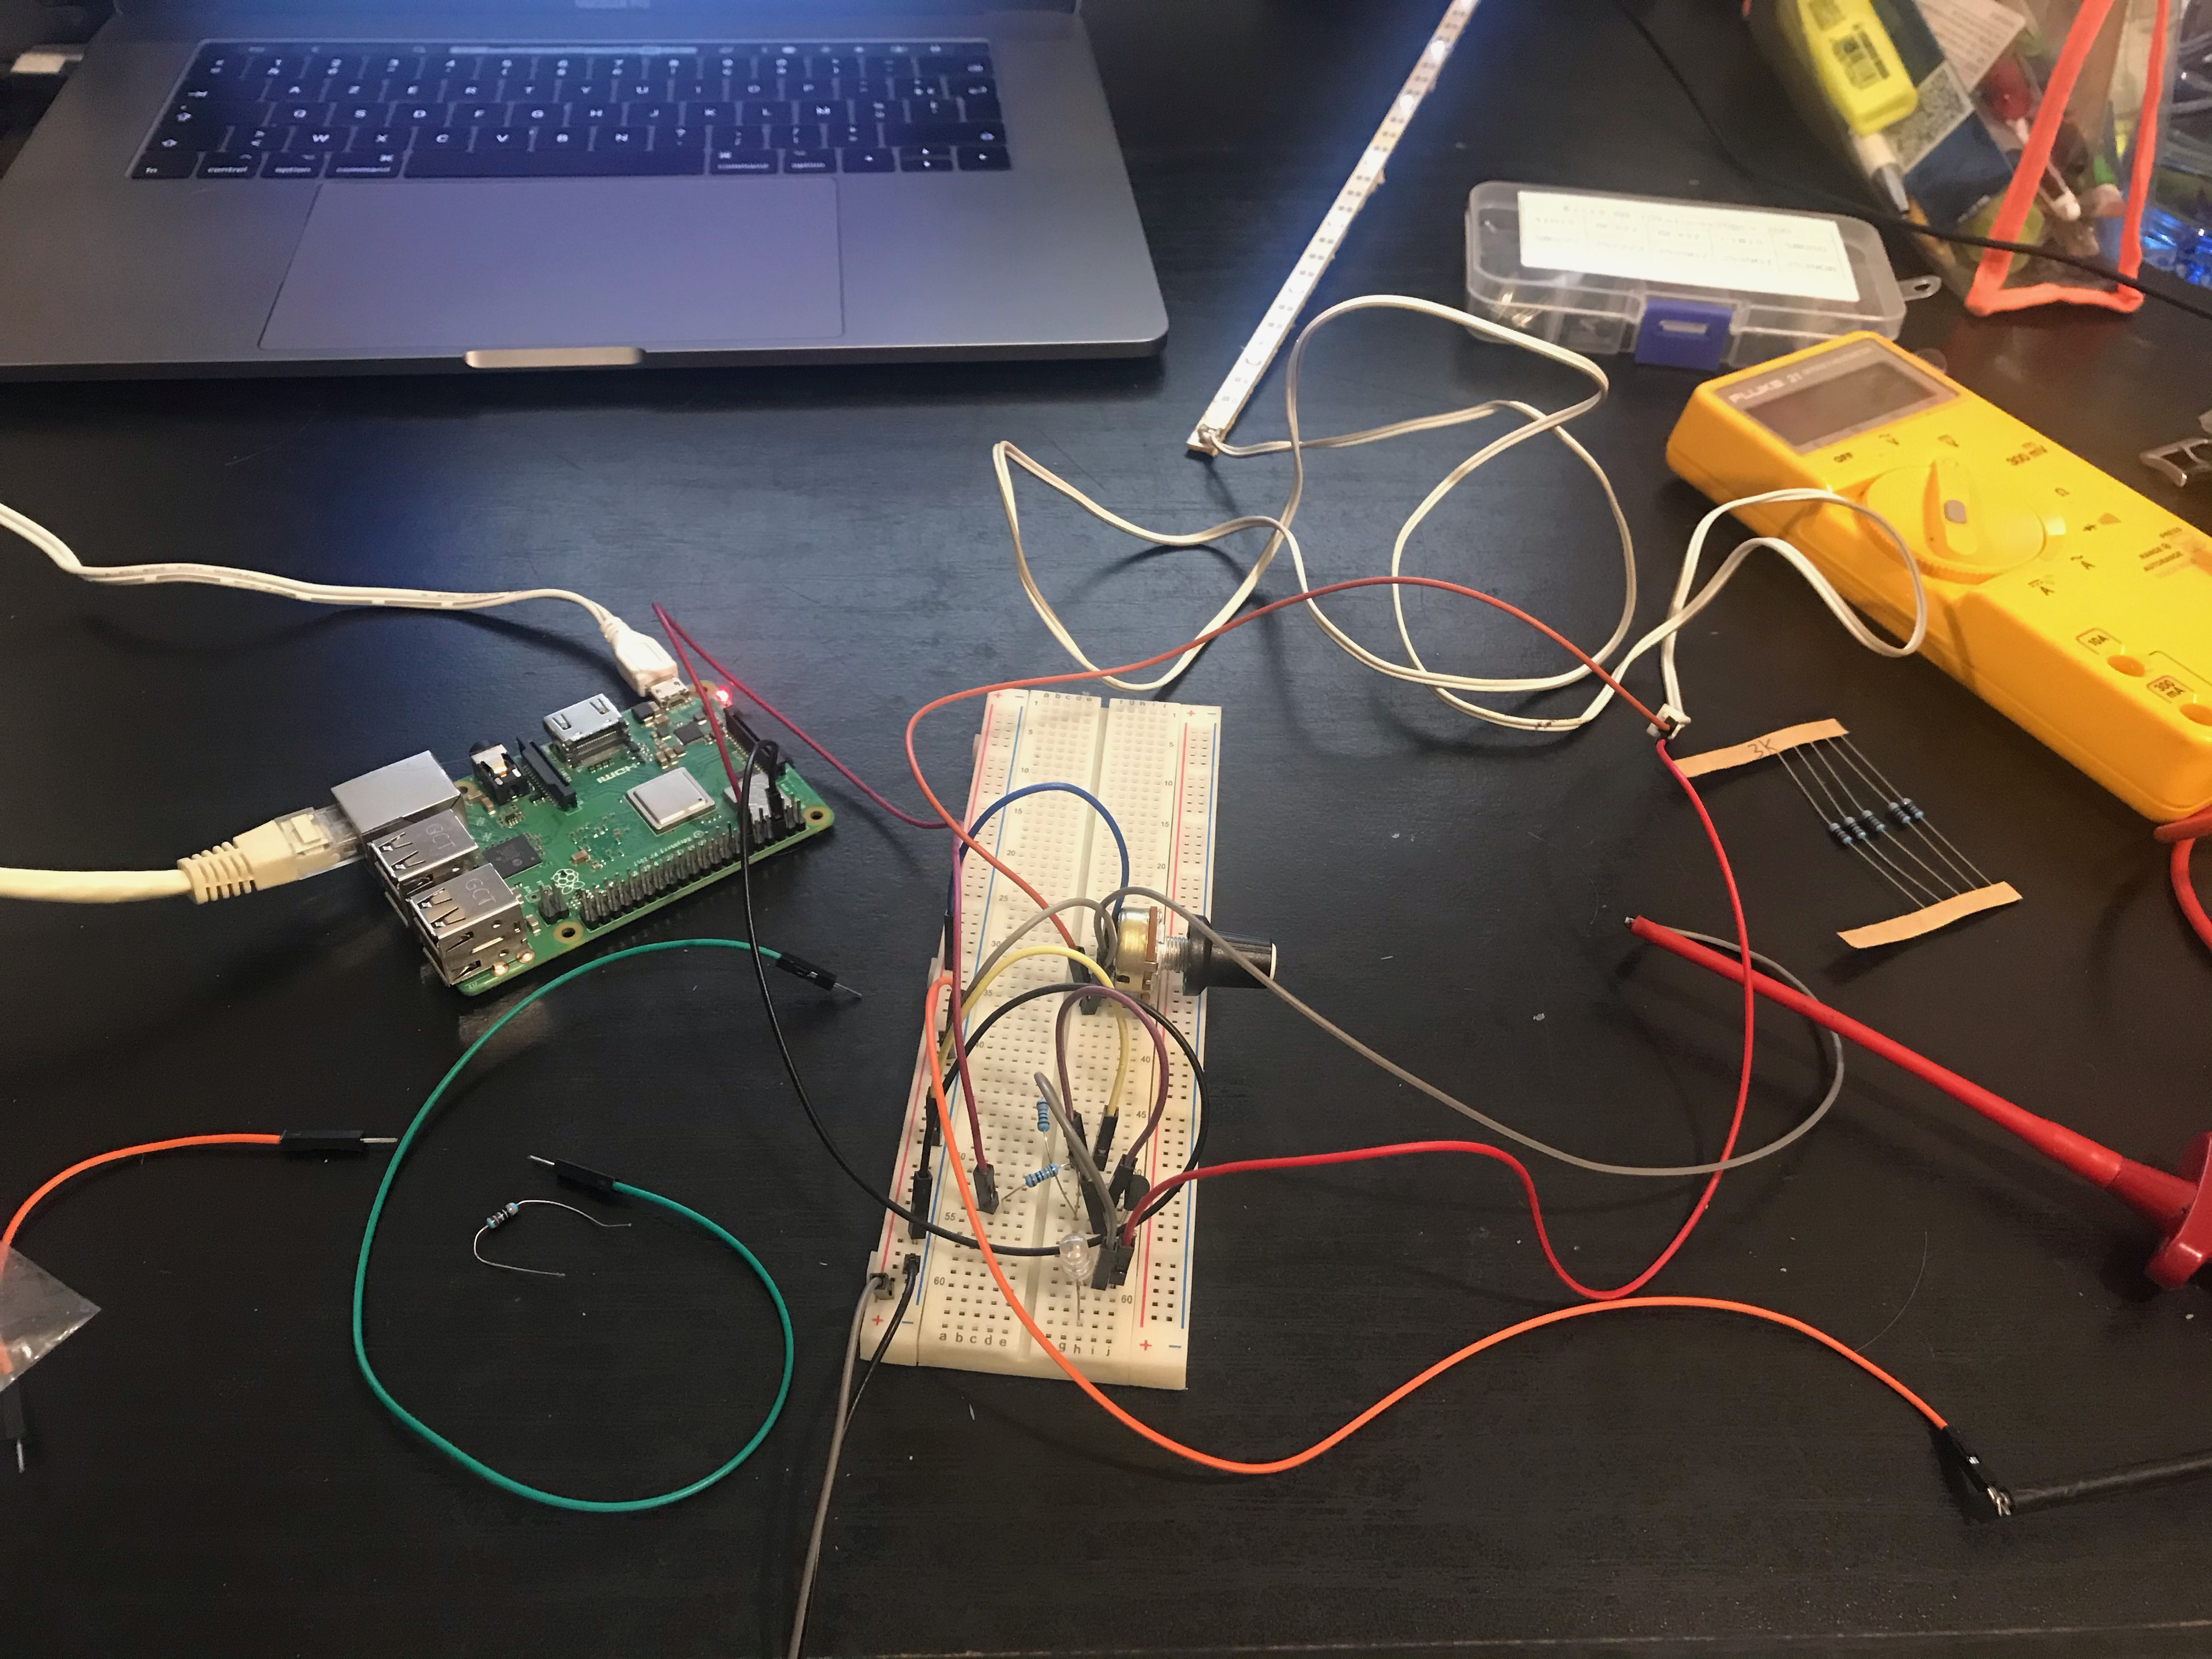
\includegraphics[width=0.5\textwidth, keepaspectratio=true]{./fig/Camera_setup/Light/White_Led_Strips/Test_setup_ledstrip.jpeg}
			\caption{White LED strips test circuit.}
			\label{fig:setup:whiteled:circuit}
		\end{figure}

	\subsubsection{Addressable Colour Changeable LED Strip}
	\label{sec:impl:camerasetup:light:ledstrips}

		A third option of lighting is playing with the colours of the light. To archive this a setup will be created with a single addressable light strip where the colour and LED can be freely chosen. 
		To assign a colour which works best; a study is made to find the wavelengths where the light reflects most on the used materials of the tool. This can be found in section \ref{sec:lit:reflection}.

From all these settings the single addressable LED strip was chosen due to the amount of options this creates. This choice is documented in future tests which will be discussed in section \ref{sec:results:spaghetti:colour}. The LED strips were mounted on metal strips which provided high adaptability. This made it possible to get lighting on different parts of the tool insert what makes later research easier. In Figure \ref{fig:impl:camerasetup:adressablestrips:reflection} the light configuration is displayed. A lot of options can be fulfilled with this set-up. Each LED strip can rotate and fifteen LEDs can be individually set to a colour. The arc keeps a consistent distance between the LED and the insert. 
	
	\begin{figure}[hbtp]
		\centering
		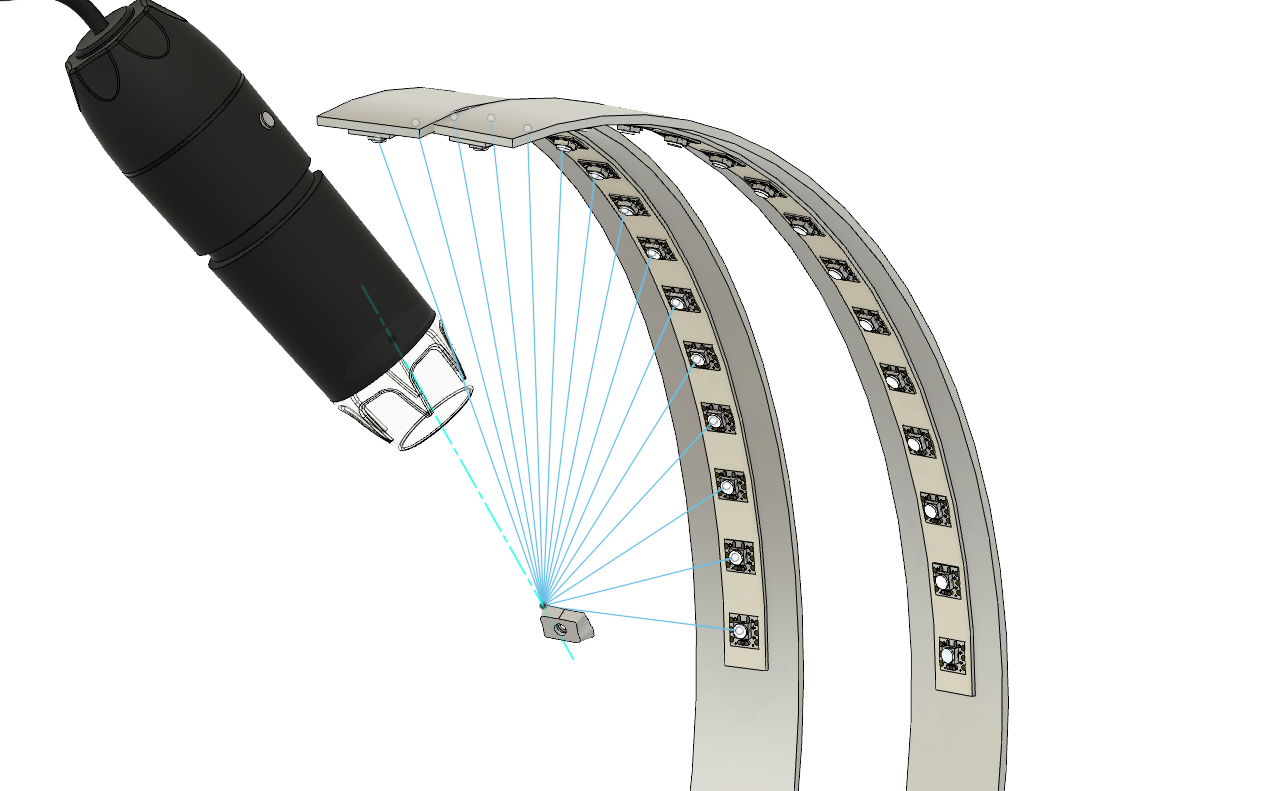
\includegraphics[width=0.49\textwidth]{fig/Camera_setup/adressable_ledstrip/ledstrips v13 close up with reflection.png}
		\caption{Visualisation of the reflections from the LED strips into the camera.}
		\label{fig:impl:camerasetup:adressablestrips:reflection}
	\end{figure}
	

\section{Datasets}
\label{sec:impl:dataset}
A separation is made between hand made datasets and automated datasets because they take a very different approach and produce very differing results.

	\subsection{Handmade datasets}

The following datasets where produced using a microscopic camera to take pictures of single inserts all placed under the camera by hand. The initial dataset is produced by Sirris.

		\subsubsection{initial dataset}

%			The initial dataset where the images made by a microscopic camera at Sirris. These pictures were taken for the measurement of the tool wear. This dataset provided labels for the first 5 batches labeled with 00x as batch number. This data was directly saved from the output of the microscopic camera. For this reason there is a lot of extra information on the picture as seen in Figure \ref{fig:dataset:initial}. The labels for this dataset where sorted with or without tag on the insert but the transcription code was lost. For example the insert had a mark on one side and no mark on the other side and the labels had a value for some insert a and some insert b. For this combination it wasn't known whether label a was the side with the mark or the other way round.
			
%			Since the labels weren't clear and the images where not optimal these inserts where all done again in a new hand made dataset called the second handmade dataset.
			
			\begin{figure}[hbtp]
			\centering
			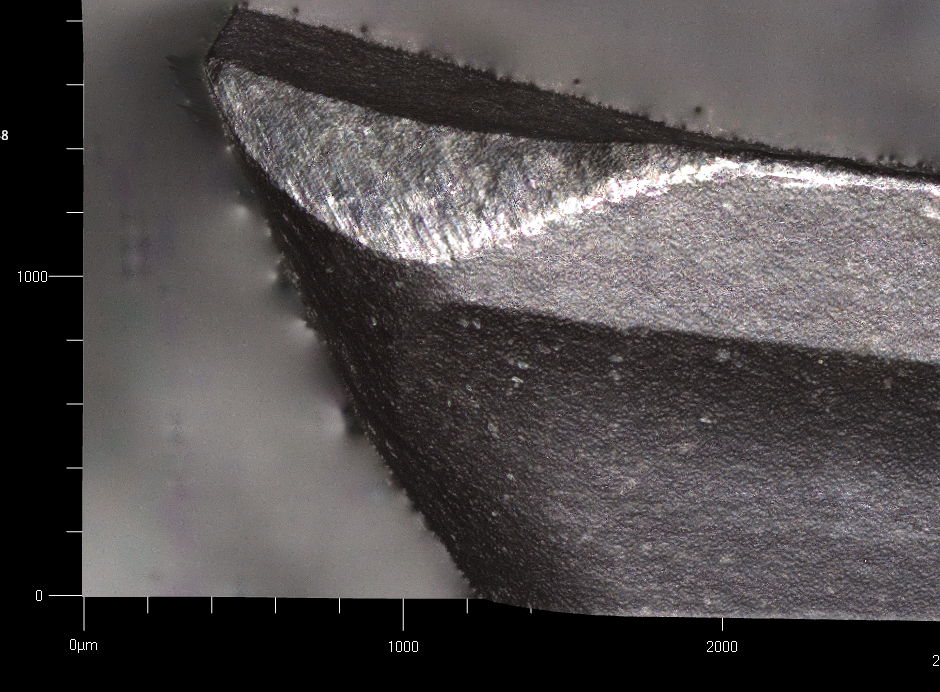
\includegraphics[scale=0.2]{fig/Vision/Dataset/handmade_datasets/initial_dataset/initial dataset pictuer.PNG}
			\caption{Example of initial dataset}
			\label{fig:dataset:initial}
			\end{figure}

%\paragraph{Form}

The dataset given where taken with a microscopic camera at Sirris. These images were in good lighting conditions for the measurement, but had a lot of extra "unwanted" features on it. The background was very like the wear and the rest of the tool insert. 

Every insert that was measured had a little mark on one side to mark the a and b side of the insert. An example of this mark is given in Figure \ref{fig:impl:va:do:mark}. Sadly the information about what the marker meant is lost. To find the corresponding values, the inserts where once again put through a microscopic camera and the new pictures where compared against the old ones. This will be discussed in the following section.

\begin{figure}[hbtp]
\centering
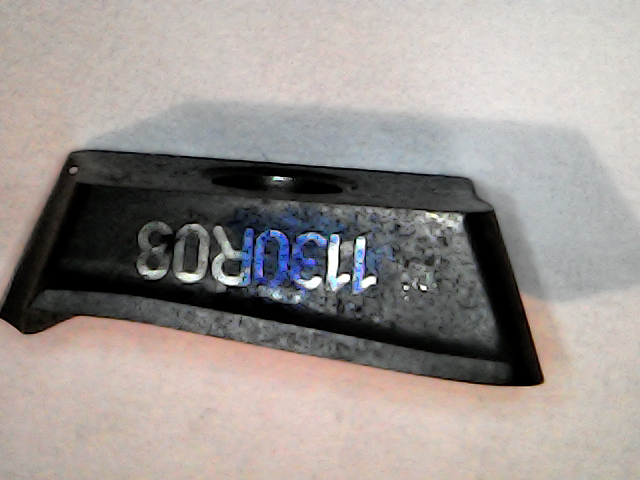
\includegraphics[width=0.3\textwidth]{fig/algemeen/plaatjes/plaatje/marked_side.jpg}
\caption{Marked side of an insert.}
\label{fig:impl:va:do:mark}
\end{figure}

			
		\subsubsection{Second handmade dataset}
		\label{sec:impl:ds:shm}
		
		%While again checking the inserts , a new dataset is created since this didn't ask much more time. During this process there is also a new way of separating the sides of the inserts. There is a bullet at one side on every insert. This is an easy way to recognise a side and wont dissapear like the marker line. This is illustrated on Figure \ref{fig:impl:va:do:bullet} where the red square marks the bullet.
		
		
\begin{figure}[hbtp]
			\centering
			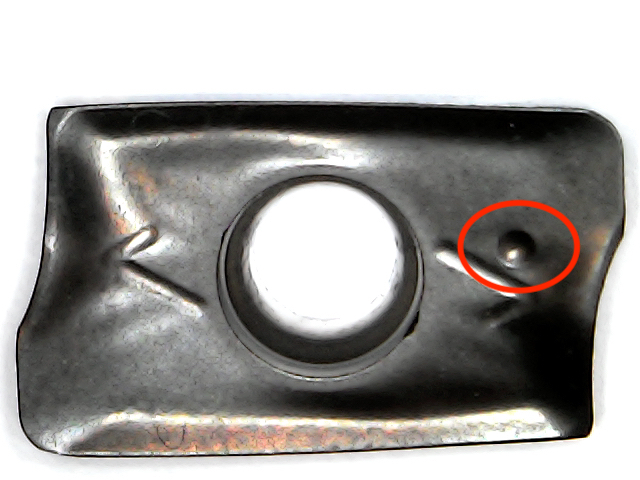
\includegraphics[width=.49\textwidth]{fig/algemeen/plaatjes/plaatje/top_view_bullet_marked.jpg}
			\caption{Bulled mark marked on the top view of an insert.}
			\label{fig:impl:va:do:bullet}
		\end{figure}

			A second dataset was made to compare the pictures with the previous dataset. This is done to verify the images and the results and to determine what the markings on the inserts meant. This dataset handles the first 5 batches labeled with 00x. For this dataset a setup was made where the insert is placed on its side on a black background with the microscope camera vertical above the insert. Only the light from the camera was used.

		During the creation of this dataset the inserts where labeled with bullet or no bullet. What we mean by bullet is marked on Figure \ref{fig:impl:va:do:bullet}. Now all labels have the following information:
		\begin{itemize}
			\item A value of tool wear.
			\item Whether the side of the insert is marked.
			\item If a bullet mark can be fount on that side of the insert.
\end{itemize}	

	Later on this bullet can be used as an universal identifier for the sides of the inserts. The most information is also stored in the name of the image. This is indicated in table \ref{tab:impl:dataset:shm:name}.
	
	\begin{table}
	\centering
	\caption{Explanation for the image names for the second handmade dataset. }
		\begin{tabular}{ |l|l| }
			\hline
 				symbol & explanation \tabularnewline
			\hline
			\hline
				 s & side with marker line \tabularnewline
			\hline
				 n & side without marker line \tabularnewline
			\hline
				 batch number & number specified on the box in which the inserts are kept \tabularnewline
			\hline
				 insert number & number specified inside the box; this goes from 1 to 10 per batch \tabularnewline
			\hline
		\end{tabular}
		\label{tab:impl:dataset:shm:name}
	\end{table}

		The naming of the dataset is as follows:

		b\_\textless{}batch number\textgreater{}\_p\_\textless{}plate number\textgreater{}\_\textless{}identifier of side\textgreater{}

		When all data images where created, we took a look ath the pictures from the dataset as specified in Figure \ref{fig:impl:va:do:comparison}.  It can now be confirmed that the two images correspond and that the 'b' side of the inserts is the side with the marker line. 

\begin{figure}[hbtp]
	\begin{subfigure}{0.49\textwidth}
			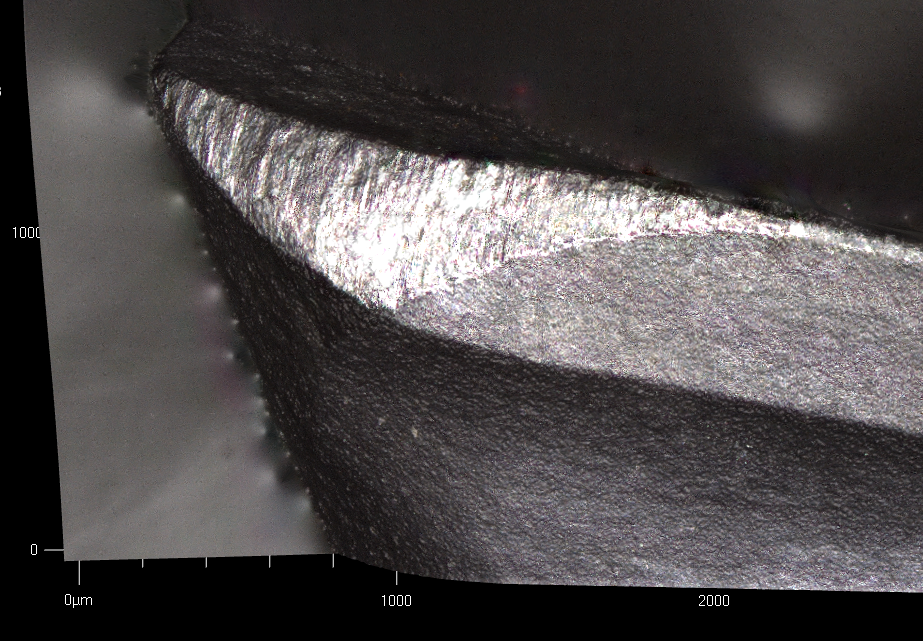
\includegraphics[width=\linewidth, keepaspectratio=true]{./fig/Vision/Dataset/handmade_datasets/Second_handmade_dataset/t50b-img.PNG}
			\caption{Image from the first initial dataset.}
		\end{subfigure}
		\begin{subfigure}{0.49\textwidth}
			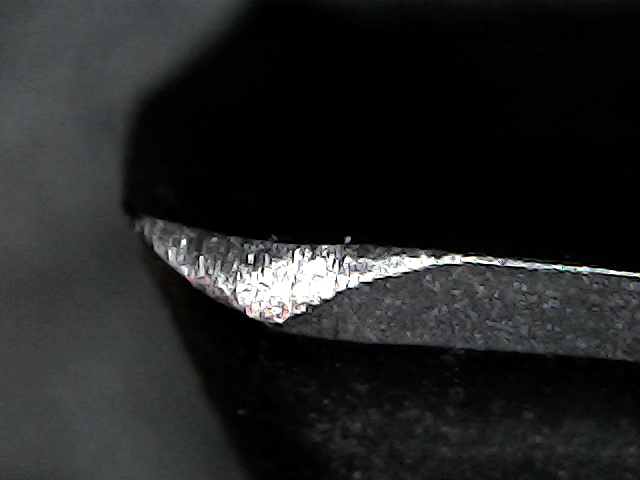
\includegraphics[width=\linewidth, keepaspectratio=true]{./fig/Vision/Dataset/handmade_datasets/Second_handmade_dataset/b_005_p_010_s.jpg}
			\caption{Image from the second handmade dataset.}
		\end{subfigure}
			\caption{Comparison of the same insert 19 from batch 5 the side with marking.}
			 \label{fig:impl:va:do:comparison}
\end{figure}
			
	
		\subsubsection{second initial dataset}

			The second initial dataset was made with the inserts from batches 11 to 19 labelled with 01x. The images where taken with the same microscope as the first initial dataset but instead of photographing only the one insert at a time, two inserts are photographed per shot.
Since the photo's where labelled with two inserts at a time, the images taken where not relevant for the data processing and were not saved.

	\subsection{Automated datasets}

	The handmade datasets are not scalable for a hundred or even a thousand inserts so a way of automatically creating datasets was researched in \ref{sec:impl:camerasetup}. When all building blocks for an automated set-up where created, a program was written to control the set-up  and save the taken images in a logical order. This process took a lot of test tries to find out a good camera position which will be handled first. After that the two created datasets will be discussed.

		\subsubsection{Camera position}
		In this section the best camera position will be defined  for the creation of the dataset. Top view as well as side view will be tested.

		\paragraph{Side camera position}

		The first four plates of batch 004 are used to test the side view camera position. The lighting is red light coming from the addressable LED strips that shine from different directions as specified in section \ref{sec:impl:camerasetup:light:ledstrips}. The practical implementation of the setup can be seen on Figure \ref{fig:dataset:cameraposition:side}.

		\begin{figure}[hbtp]
			\centering
			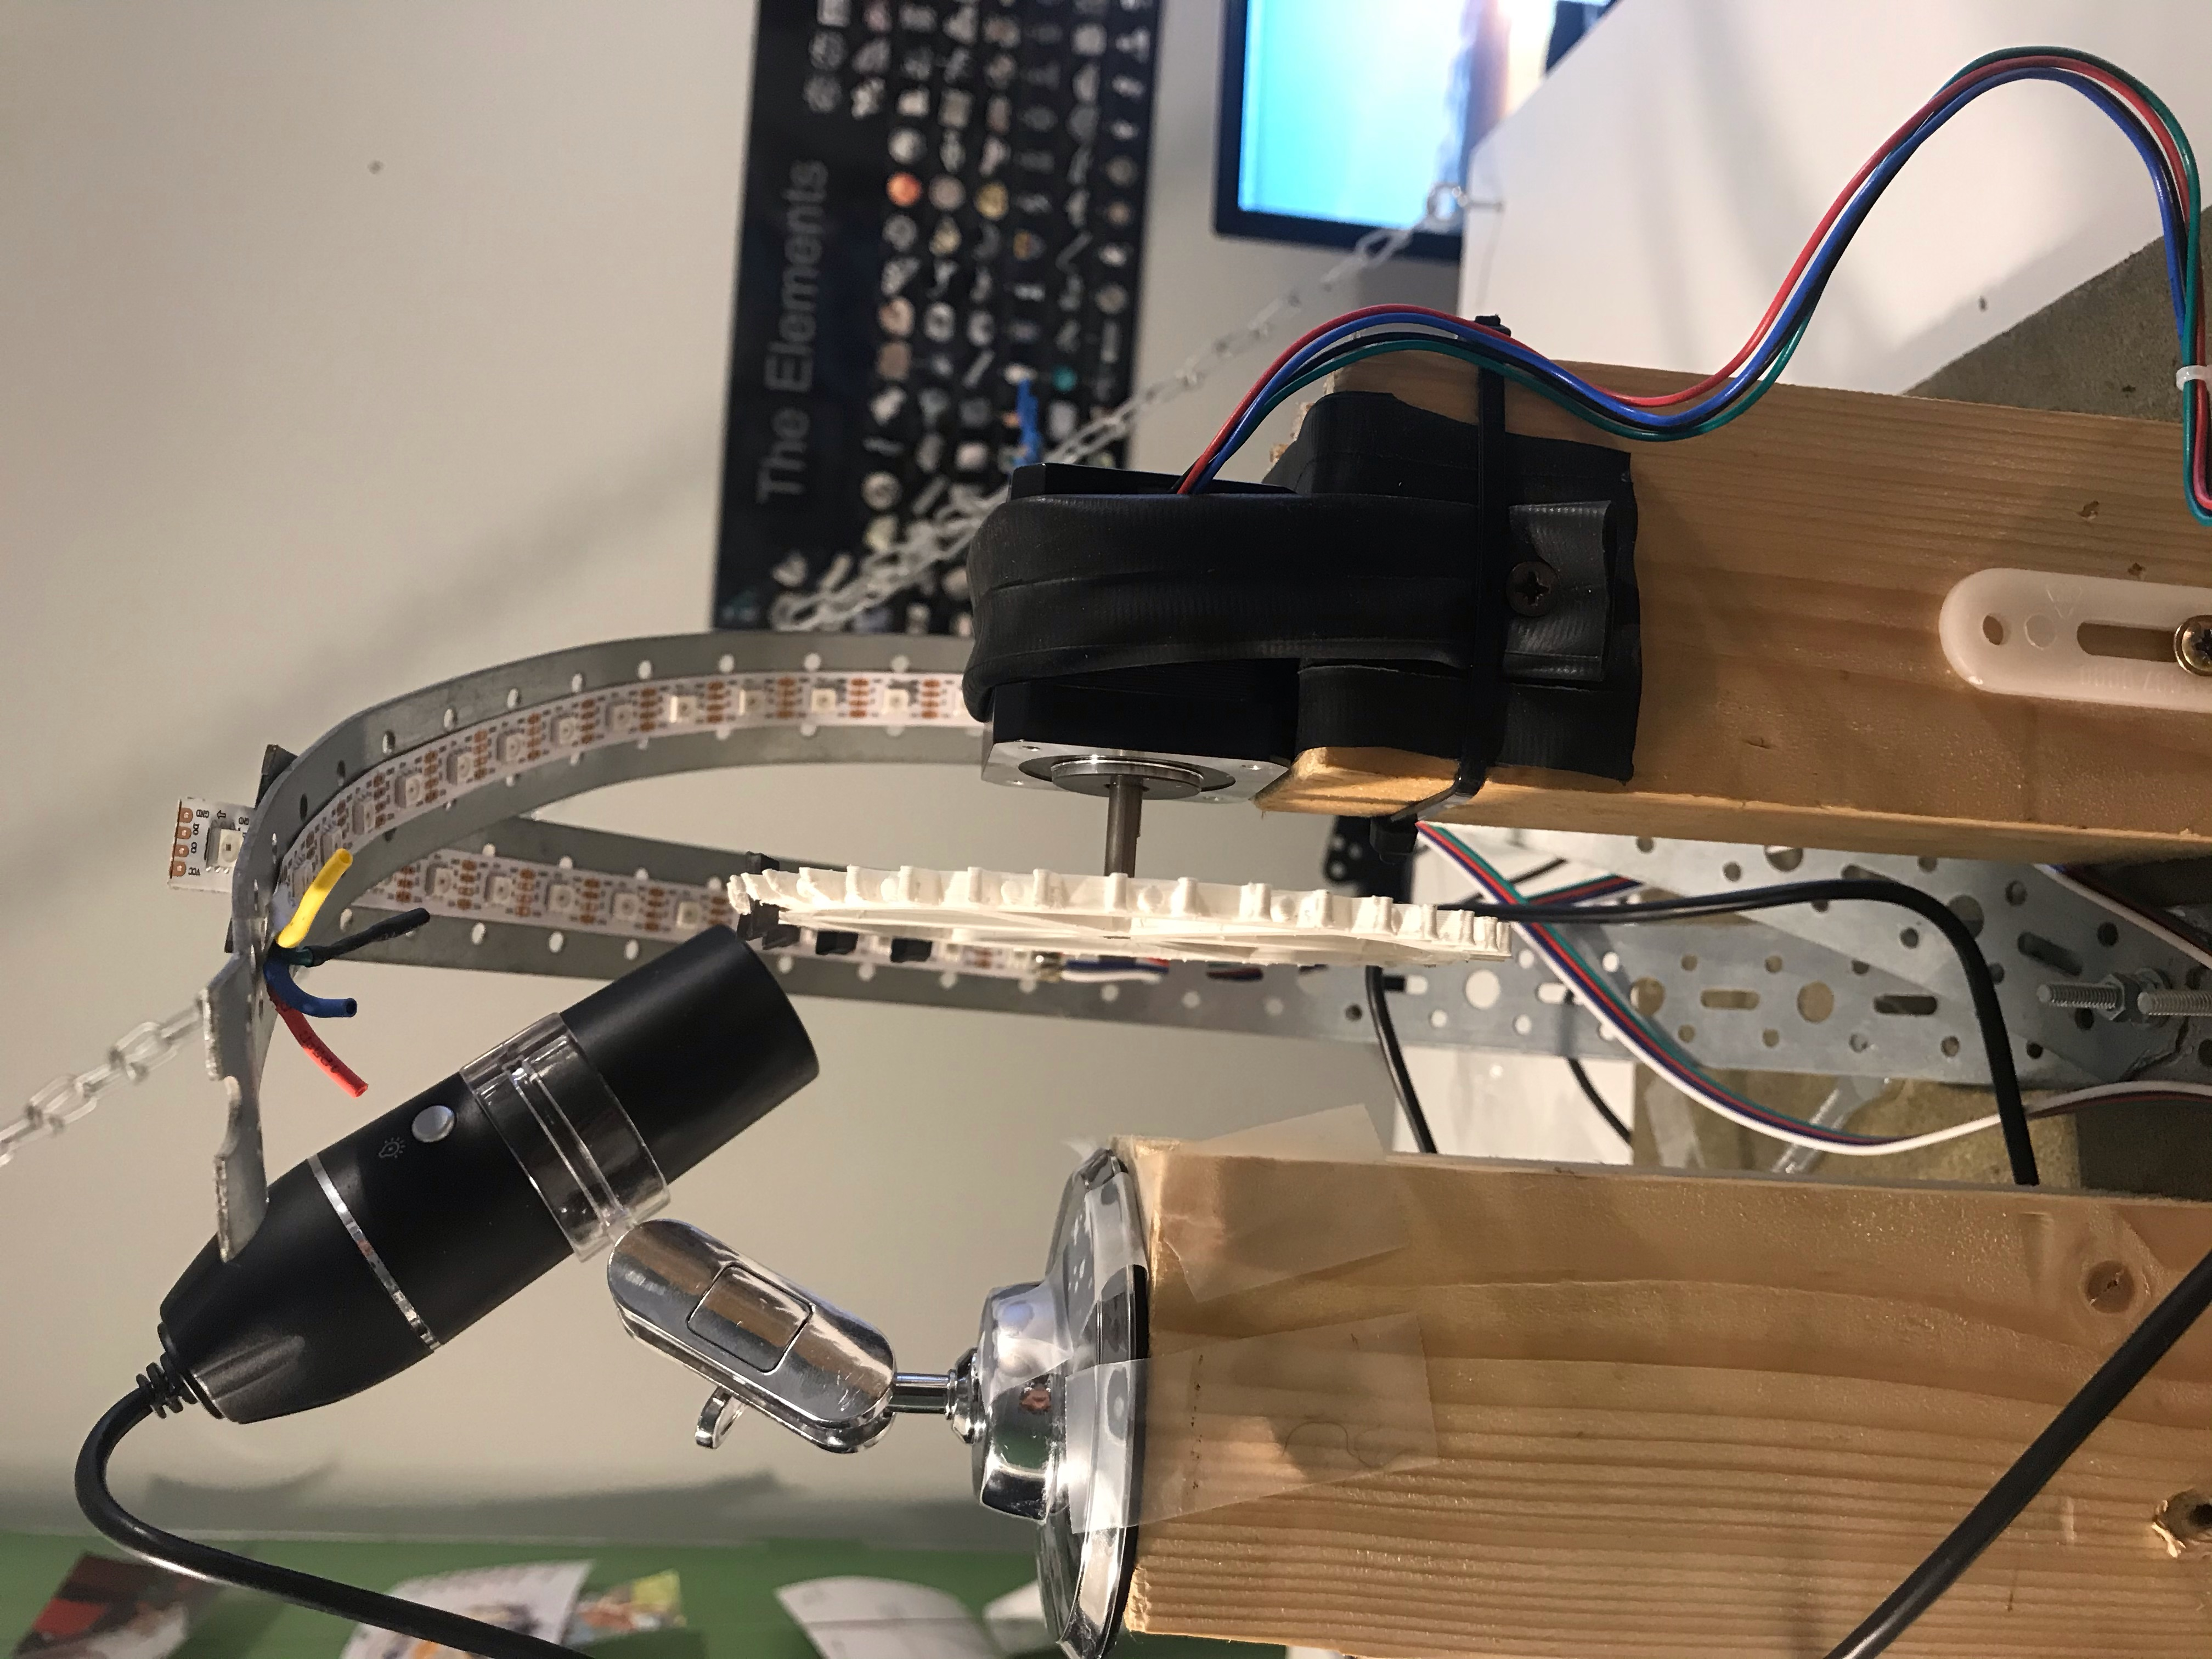
\includegraphics[width=0.49\textwidth, keepaspectratio=true,angle=270]{./fig/Vision/Dataset/automated_datasets/1_check_camera_position/1_camera_position_side/achter2.jpeg}
			\caption{Camera setup for testing the camera angle.}
			\label{fig:dataset:cameraposition:side}
		\end{figure}

		During the creation of the dataset, there where some problems with the microprocessor that controlled the lights. It would take one full second to process a command send by the computer connected to it. This resulted in an unsuccessful test because the LEDs didn't turn on when the photo's where taken. The produced images where all black with a little shadow of the insert caused by the polluting light from the room. 

		The error was temporarily resolved by putting a delay before sending a command to the micro processor to provide the wanted lighting conditions. Although this was a very long process the results are way better than the ones from the first take on this camera set-up. 

		These can be found in Figure \ref{fig:dataset:cameraposition:side:results}. The insert is lighted with two corresponding LEDs coming from the two LED strips described in \ref{sec:impl:camerasetup:light:ledstrips}. On the left is the result for LED number 8; in the middle LED number 9 and on the right LED number 10. This lightens the worn area very good. Although the background is lighted as well and makes it harder to only see the worn area. Nevertheless can we build the first dataset with this. First the top camera view is tested.

		\begin{figure}
			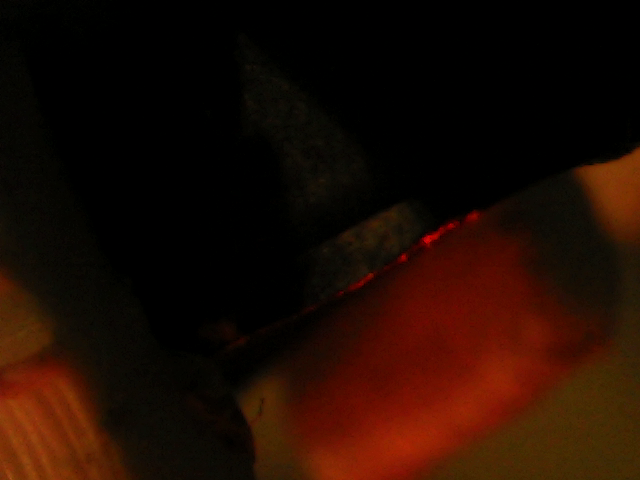
\includegraphics[width=.3\textwidth, keepaspectratio=true]{./fig/Vision/Dataset/automated_datasets/1_check_camera_position/1_camera_position_side/p3_l8.png}\hfill
			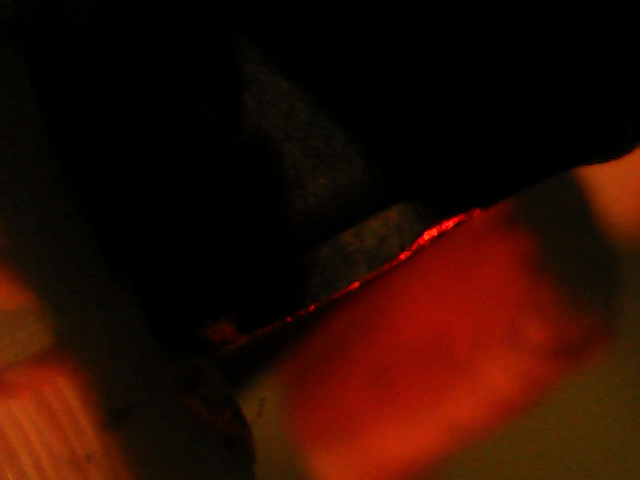
\includegraphics[width=.3\textwidth, keepaspectratio=true]{./fig/Vision/Dataset/automated_datasets/1_check_camera_position/1_camera_position_side/p3_l9.png}\hfill
			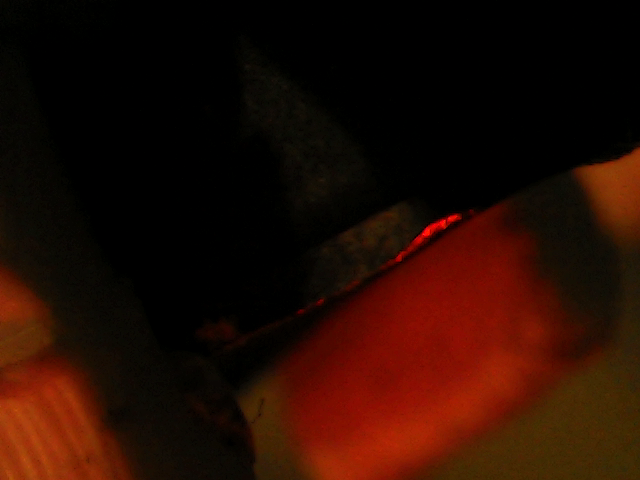
\includegraphics[width=.3\textwidth, keepaspectratio=true]{./fig/Vision/Dataset/automated_datasets/1_check_camera_position/1_camera_position_side/p3_l10.png}
			\caption{Side camera view for LED 8 through 10 listed from left to right.}
			\label{fig:dataset:cameraposition:side:results}
		\end{figure}

		\paragraph{Top camera position}

A second test was conducted with the camera mounted a little more to the top of the inserts. This made the reflection from the worn area to the camera better. 
%For this test the same inserts where used (batch 4 insert 1 to 5). Like the side view test, every pair of LEDs is lighted separately to generate the photo's. 

For this test the issue with the micro processor communication was resolved by changing the input delay from the serial input reader. The resulting pictures can be found in Figure \ref{fig:dataset:cameraposition:top:results}.
Like on the previous test one picture was taken for every two LEDs of the strip with red light. This was done for batch number 4 insert 3 this time with LEDs 5,6 and 7 turned on since the position of the camera relative to the LEDs changed.

\begin{figure}
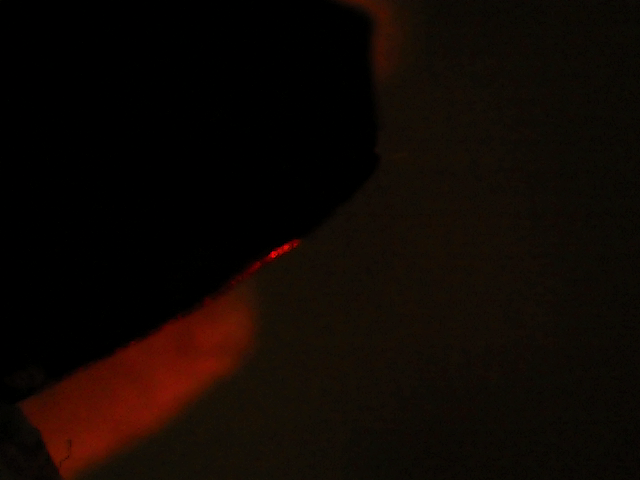
\includegraphics[width=0.32\textwidth, keepaspectratio=true]{./fig/Vision/Dataset/automated_datasets/1_check_camera_position/2_camera_position_top/p3_l5.png}\hfill
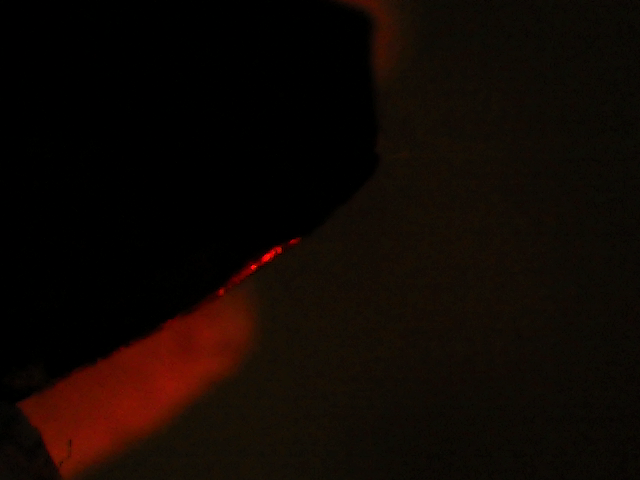
\includegraphics[width=.32\textwidth, keepaspectratio=true]{./fig/Vision/Dataset/automated_datasets/1_check_camera_position/2_camera_position_top/p3_l6.png}\hfill
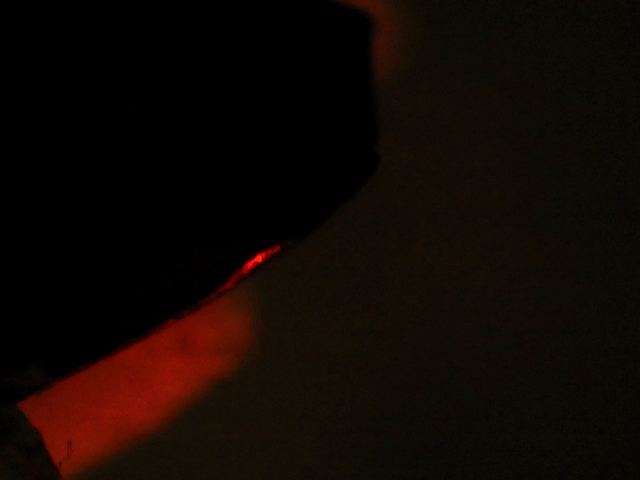
\includegraphics[width=.32\textwidth, keepaspectratio=true]{./fig/Vision/Dataset/automated_datasets/1_check_camera_position/2_camera_position_top/p3_l7.png}
\caption{Top camera view for LEDs 5 through 7 listed from left to right.}
\label{fig:dataset:cameraposition:top:results}
\end{figure}

On this data we can see the LEDs going up on the insert wear area. Which is what we tried to obtain. Now the LEDs are mapped to specific positions on the inserts and the amount of LEDs that need to be turned on for taking pictures can be reduced so no extra time is wasted. 

		\subsection{Created datasets}

The full datasets will be discussed in this section where we start with a brief explanation of the dataset and proceed with a view of the set-up after which the results are illustrated.

			\subsubsection{Birthday dataset}
			\label{sec:impl:dataset:birthday}
			
			The first full dataset is the Birthday dataset which was meant to take a picture of every insert with all possible lighting settings. After the first 6 batches the output was inspected and the process was halted. The process will be discussed in the next paragraphs.
		

			\paragraph{Dataset explanation}
			The birthday dataset was created on 27/11/2020 with a part of the given inserts for every possible colour and led setting where pictures are taken from inserts using the two separate LED strips where every LED is turned on separately. This is done for white, red, green and blue colours as listed below. This results in a total of 91 images per insert side.

			\begin{itemize}
				\item 1 picture with all LEDs on white
				\item 30 pictures with red lighting; 15 of LED strip A and 15 of LED strip B
				\item 30 pictures with blue lighting; 15 of LED strip A and 15 of LED strip B
				\item 30 pictures with green lighting; 15 of LED strip A and 15 of LED strip B
			\end{itemize}

			%The dataset consists of 120*91 photos of 60 inserts with 120 worn sides. After 120 the quality was evaluated and the red, green and blue colours didn't seem to add more information to the pictures. 


			\paragraph{Set-up}
			Two ledstrips where mounted and pointed at the photographed insert. The brightness is set to 80\% for all LEDs to make sure to not clip against the saturation values for the pixels. The inserts where attached to the wheel from \ref{sec:impl:camerasetup:wheelholder} with black clips 3D printed with PETG. This was chosen above white clips to lower the light reflections into the camera. This was a problem in previous set-ups.
			Also the sturdy camera mount from section \ref{sec:impl:camerasetup:cameramount} was used to get better notice of the placement of the camera opposed to the insert. 

			\paragraph{Results}
			The image taking process took about 1 minute per insert because of the amount of pictures taken. Since time was limited and the set-up wasn't yet perfect we decided to only run 60 inserts. These where from batches 1 to 11. 

			Sample pictures of this dataset can be found in Figures \ref{fig:impl:dataset:birthday:strip1} and \ref{fig:impl:dataset:birthday:strip2}. Where \ref{fig:impl:dataset:birthday:strip1} are images from LED strip 1 and \ref{fig:impl:dataset:birthday:strip2} are images from LED strip 2. We can see that LED strip 1 wasn't configured well where it resulted in all black pictures. For LED strip one we can asses the use of colours. Only white and red are really visible, blue and green are not visible on the images thus these colours won't be used for later research.



			\begin{figure}[hbtp]
				\centering
				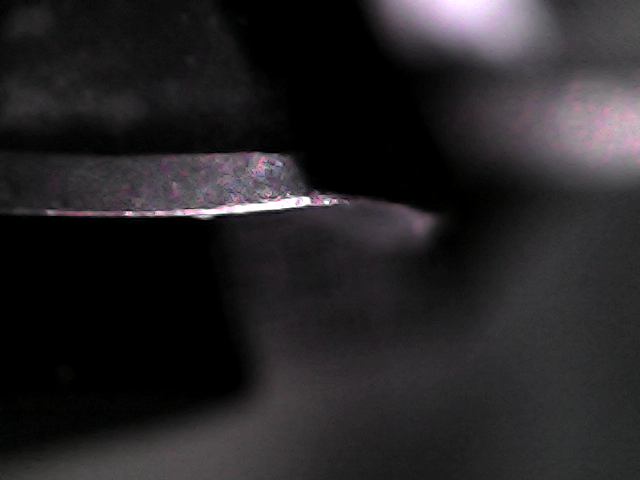
\includegraphics[width=.3\textwidth, keepaspectratio=true]{./fig/Vision/Dataset/automated_datasets/2_created_datasets/1_Birthday_dataset/b_003_p_005_l_000_b.png}
				\caption{Fully lit example for insert 5 from batch 3.}
			\end{figure}

			\begin{figure}
				\begin{subfigure}{0.24\textwidth}
					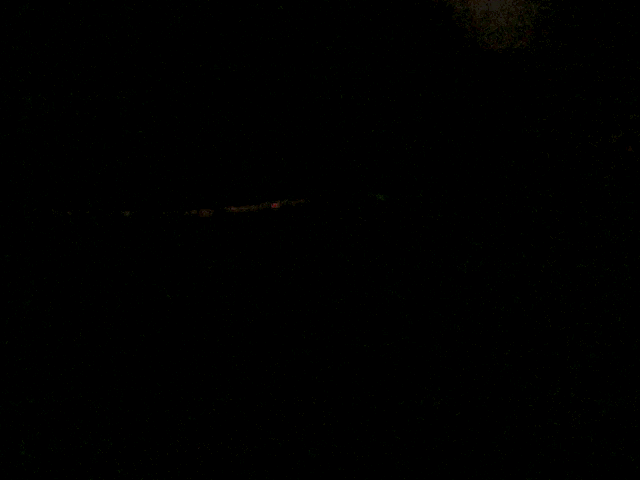
\includegraphics[width=\linewidth, keepaspectratio=true]{./fig/Vision/Dataset/automated_datasets/2_created_datasets/1_Birthday_dataset/b_003_p_005_b_l_006_red_A.png}
					\caption{Red}
				\end{subfigure}
				\hspace*{\fill}
				\begin{subfigure}{0.24\textwidth}
					
\includegraphics[width=\linewidth, keepaspectratio=true]{./fig/Vision/Dataset/automated_datasets/2_created_datasets/1_Birthday_dataset/b_003_p_005_b_l_006_green_A.png}
					\caption{Green}
				\end{subfigure}
				\hspace*{\fill}
				\begin{subfigure}{0.24\textwidth}
					
\includegraphics[width=\linewidth, keepaspectratio=true]{./fig/Vision/Dataset/automated_datasets/2_created_datasets/1_Birthday_dataset/b_003_p_005_b_l_006_blue_A.png}
					\caption{Blue}
				\end{subfigure}
				\hspace*{\fill}
				\begin{subfigure}{0.24\textwidth}
					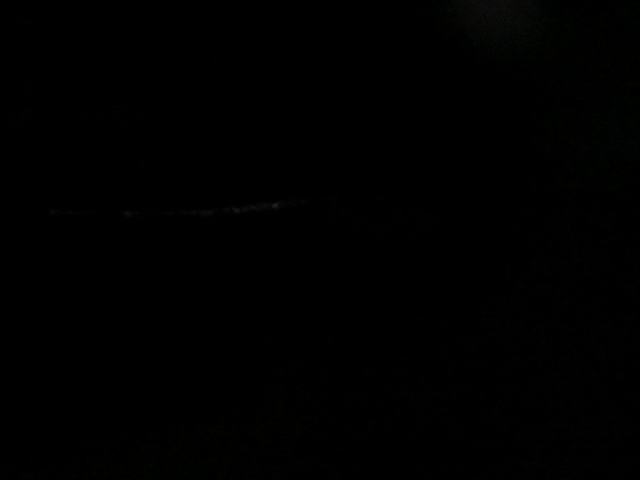
\includegraphics[width=\linewidth, keepaspectratio=true]{./fig/Vision/Dataset/automated_datasets/2_created_datasets/1_Birthday_dataset/b_003_p_005_b_l_006_white_A.png}
					\caption{White}
				\end{subfigure}
			\caption{Red, green, blue and white lighting on insert 5 from batch 3 LED strip one. Left to right respectively}
			\label{fig:impl:dataset:birthday:strip1}
		\end{figure}

		\begin{figure}
			\begin{subfigure}{0.24\textwidth}
				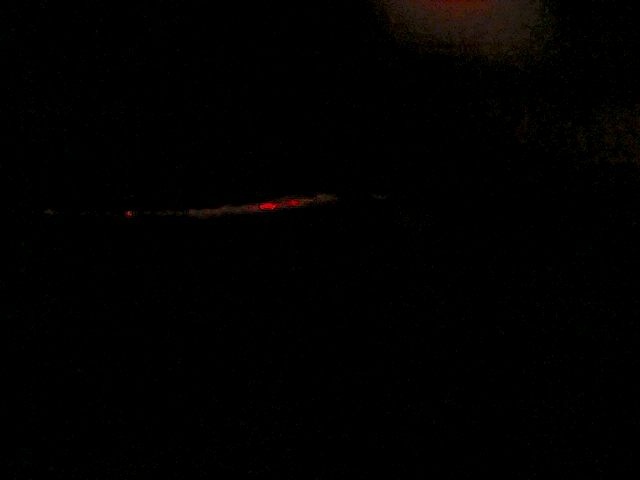
\includegraphics[width=\linewidth, keepaspectratio=true]{./fig/Vision/Dataset/automated_datasets/2_created_datasets/1_Birthday_dataset/b_003_p_005_b_l_006_red_B.png}
				\caption{Red}
			\end{subfigure}
			\hspace*{\fill}
			\begin{subfigure}{0.24\textwidth}
				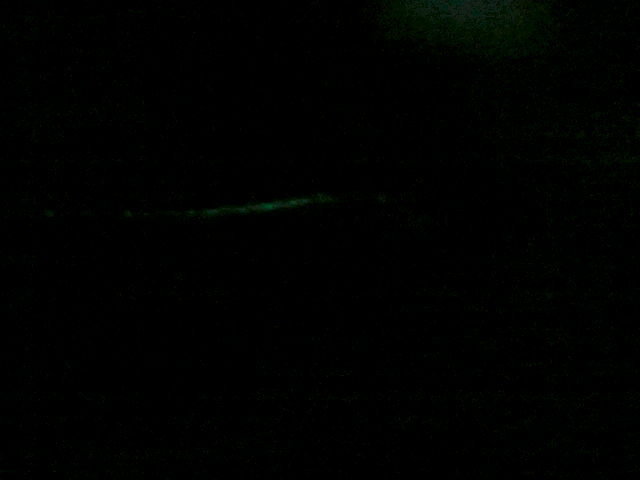
\includegraphics[width=\linewidth, keepaspectratio=true]{./fig/Vision/Dataset/automated_datasets/2_created_datasets/1_Birthday_dataset/b_003_p_005_b_l_006_green_B.png}
				\caption{Green}
			\end{subfigure}
			\hspace*{\fill}
			\begin{subfigure}{0.24\textwidth}
				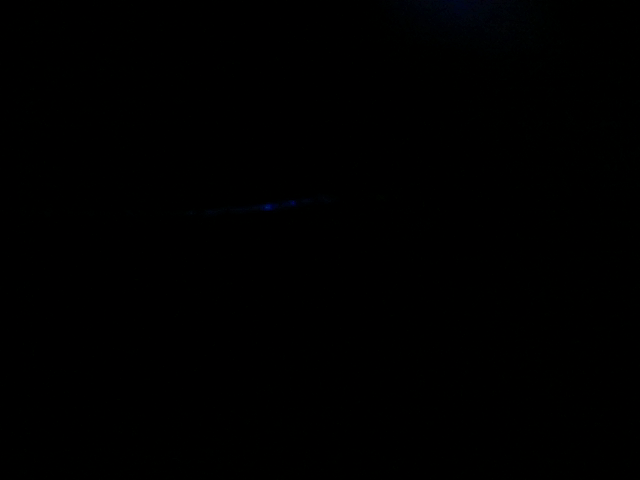
\includegraphics[width=\linewidth, keepaspectratio=true]{./fig/Vision/Dataset/automated_datasets/2_created_datasets/1_Birthday_dataset/b_003_p_005_b_l_006_blue_B.png}
				\caption{Blue}
			\end{subfigure}
			\hspace*{\fill}
			\begin{subfigure}{0.24\textwidth}
				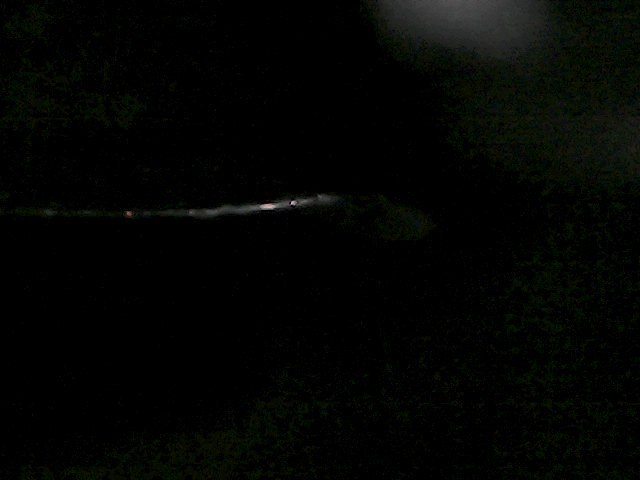
\includegraphics[width=\linewidth, keepaspectratio=true]{./fig/Vision/Dataset/automated_datasets/2_created_datasets/1_Birthday_dataset/b_003_p_005_b_l_006_white_B.png}
				\caption{White}
			\end{subfigure}
			\caption{Red, green, blue and white lighting on insert 5 from batch 3 LED strip two. Left to right respectively.}
			\label{fig:impl:dataset:birthday:strip2}

		\end{figure}


In this dataset, there are some pictures unusable, an overview of the errors is given in Figure \ref{fig:dataset:birthday:error}. As some worn areas are not even in the frame. Some to the left side (Figure\ref{fig:impl:dataset:birthday:error:left}) and some to the right side (Figure \ref{fig:impl:dataset:birthday:error:left}). 
On \ref{fig:impl:dataset:birthday:error:plastic} we see a little plastic that was still on the insert which blocks the view of the wear area. This must be cleaned before conducting a new dataset. On \ref{fig:impl:dataset:birthday:error:light} the lighting is not correctly reflected into the camera.

\begin{figure}[hbtp]
	\begin{subfigure}{0.24\textwidth}
		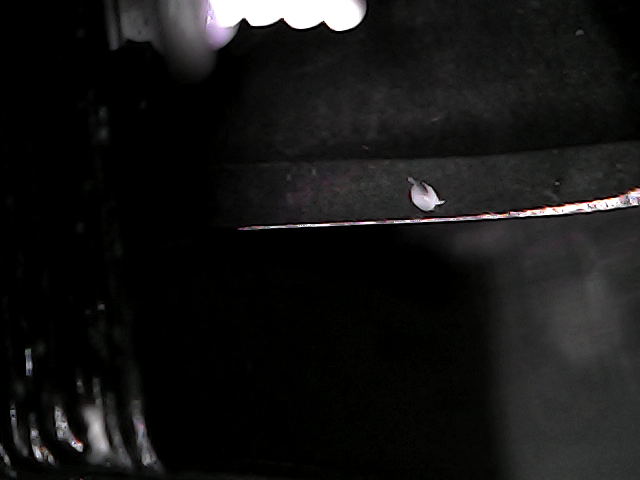
\includegraphics[width=\linewidth, keepaspectratio=true]{./fig/Vision/Dataset/automated_datasets/2_created_datasets/1_Birthday_dataset/b_003_p_010_l_000_nb.png}
		\caption{Insert out of frame left.}
		\label{fig:impl:dataset:birthday:error:left}
	\end{subfigure}
	\hspace*{\fill}
	\begin{subfigure}{0.24\textwidth}
		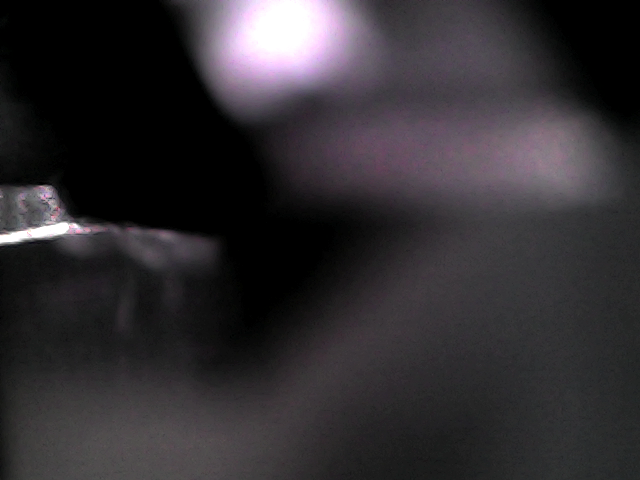
\includegraphics[width=\linewidth, keepaspectratio=true]{./fig/Vision/Dataset/automated_datasets/2_created_datasets/1_Birthday_dataset/b_003_p_010_l_000_b.png}
		\caption{Insert out of frame right.}
		\label{fig:impl:dataset:birthday:error:right}
	\end{subfigure}
	\hspace*{\fill}
	\begin{subfigure}{0.24\textwidth}
		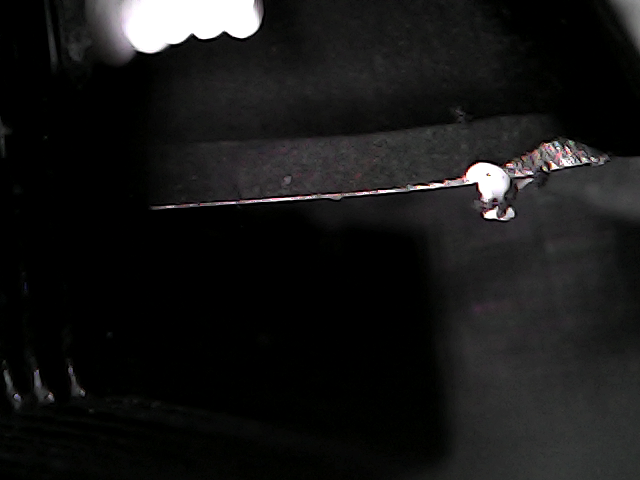
\includegraphics[width=\linewidth, keepaspectratio=true]{fig/Vision/Dataset/automated_datasets/2_created_datasets/1_Birthday_dataset/error/b_003_p_007_l_000_nb.png}
		\caption{Plastic on insert.}
		\label{fig:impl:dataset:birthday:error:plastic}
	\end{subfigure}
	\hspace*{\fill}
	\begin{subfigure}{0.24\textwidth}
		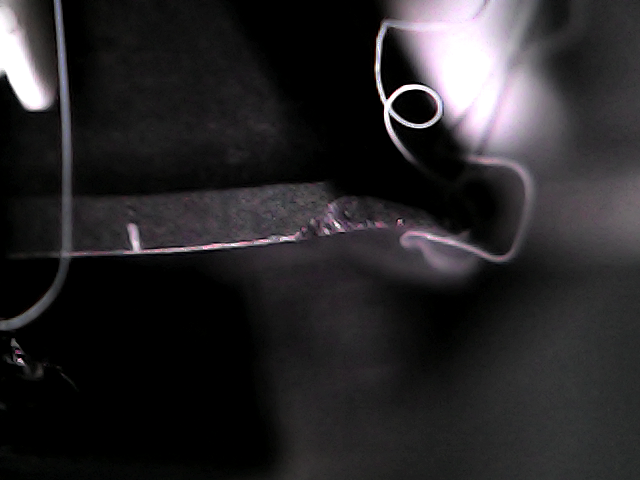
\includegraphics[width=\linewidth, keepaspectratio=true]{fig/Vision/Dataset/automated_datasets/2_created_datasets/1_Birthday_dataset/error/b_005_p_006_l_000_b.png} 
		\caption{Bad lighting angle and plastic.}
		\label{fig:impl:dataset:birthday:error:light}
	\end{subfigure}
	\caption{Errors in the Birthday dataset.}
\label{fig:dataset:birthday:error}
\end{figure}


\subsubsection{spaghetti dataset}

After the Birthday dataset a new dataset was created implementing the things learned from it. The amount of LED's driven is reduced to 5 LED's. Where LED 6 to 11 is used to lighten the inserts. 

Only colours white and red are used which was also discussed in section \ref{sec:lit:surface} that the red colour could have an influence on the reflection of the carbide of which the inserts are made.

\paragraph{Dataset explanation}

For every insert, two pictures are taken. One with LEDs 6 to 11 on red and one with these LEDs white. This was experimentally found to be the best setting for reflecting the light off the worn area and into the camera. 

The choice of turned on LEDs is important because turning on a LED to much on the upper boundary will lighten the side of the insert which isn't of much use in this research. Turning on a LED to much on the bottom boundary makes the background very bright which would provide unnecessary information.
The images are separated in a folder for every insert named with batch number and insert number:
batch\_aaa\_plate\_bbb where aaa is the batch number and bbb is the insert number.

Images are named with their settings, batch number and insert number:
b\_aaa\_p\_bbb\_l\_006-011\_color\_bullet.png 
In this name, the following fields are used:

\begin{itemize}
\item aaa is the batch number; 
\item bbb is the plate number, 
\item 006-011 are the LEDs that turned on at the same time; 
\item colour is the colour: red or white
\item bullet is the appearance of a bullet on the side of the inset and has values of b for bullet or nb for no bullet.
\end{itemize}



\paragraph{Different insert types}
The dataset inserts consisted of a few different types and coatings. These will be displayed in Figure \ref{fig:impl:datasets:spaghetti:types}. The types are listed underneath, we can distinguish two form factors and four different colours.

\begin{enumerate}[a]
	\item Grey inserts with very visible wear. These are seen in batches 1 to 5 consistently. This type will be called grey inserts. (\ref{fig:impl:datasets:spaghetti:grey})
	\item Rounded grey inserts that have a different shape on the cutting part.  (\ref{fig:impl:datasets:spaghetti:roundedgrey})
	\item Rounded black inserts with a coating that results in way darker pictures.  (\ref{fig:impl:datasets:spaghetti:roundedblack})
	\item Rounded copper inserts that have a very differing wear to the other inserts. This seems much more brittle than the other inserts.
	\item Gold coated inserts with a high reflectance.
\end{enumerate}

\begin{figure}[hbtp]
	\centering
	\begin{subfigure}{0.31\textwidth}
		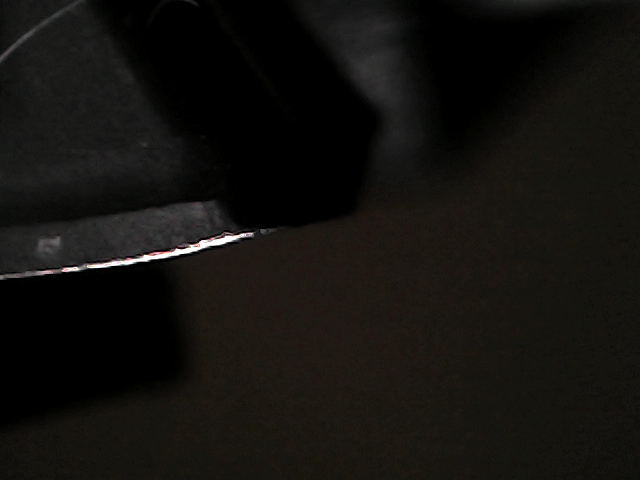
\includegraphics[width=\linewidth, keepaspectratio=true]{./fig/Vision/Dataset/automated_datasets/2_created_datasets/2_Spaghetti_dataset/gray_b_003_p_004_l_006-011_white_nb.png}
		\caption{Grey insert with very visible wear.}
		\label{fig:impl:datasets:spaghetti:grey}
	\end{subfigure}
	\hspace*{\fill}
	\begin{subfigure}{0.31\textwidth}
		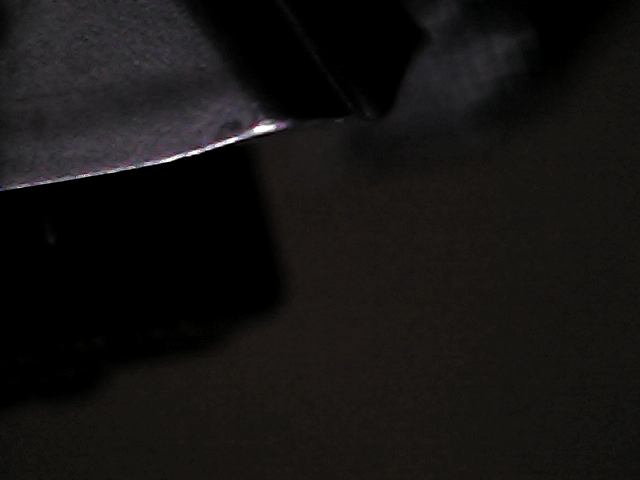
\includegraphics[width=\linewidth, keepaspectratio=true]{./fig/Vision/Dataset/automated_datasets/2_created_datasets/2_Spaghetti_dataset/rounded_grey_b_011_p_008_l_006-011_white_nb.png}
		\caption{Rounded grey insert.}
		\label{fig:impl:datasets:spaghetti:roundedgrey}
	\end{subfigure}
	\hspace*{\fill}
	\begin{subfigure}{0.31\textwidth}
		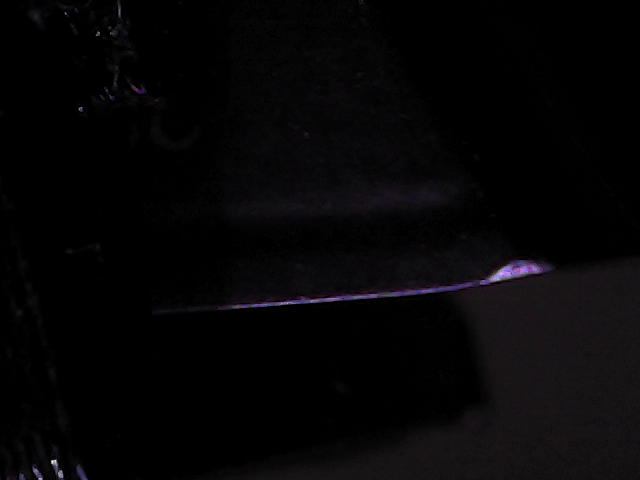
\includegraphics[width=\linewidth, keepaspectratio=true]{./fig/Vision/Dataset/automated_datasets/2_created_datasets/2_Spaghetti_dataset/rounded_black_b_013_p_002_l_006-011_white_nb.png}
		\caption{Rounded black insert.}
		\label{fig:impl:datasets:spaghetti:roundedblack}
	\end{subfigure}
	\hspace*{\fill}
	\begin{subfigure}{0.31\textwidth}
		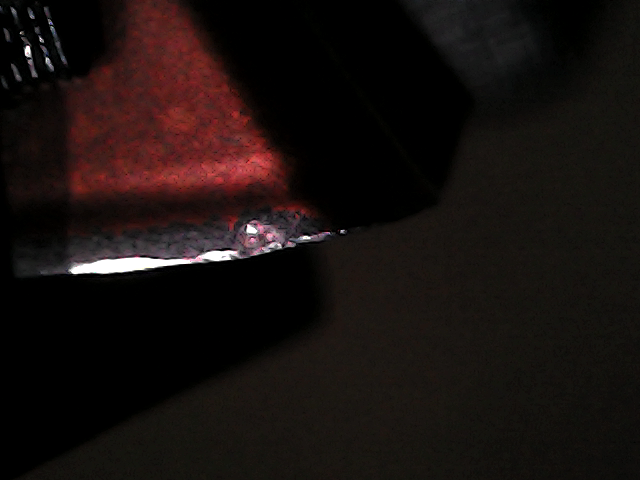
\includegraphics[width=\linewidth, keepaspectratio=true]{./fig/Vision/Dataset/automated_datasets/2_created_datasets/2_Spaghetti_dataset/rounded_copper_b_014_p_005_l_006-011_white_nb.png}
		\caption{Copper coloured insert.}
		\label{fig:impl:datasets:spaghetti:copper}
	\end{subfigure}
	\hspace*{\fill}
	\begin{subfigure}{0.31\textwidth}
		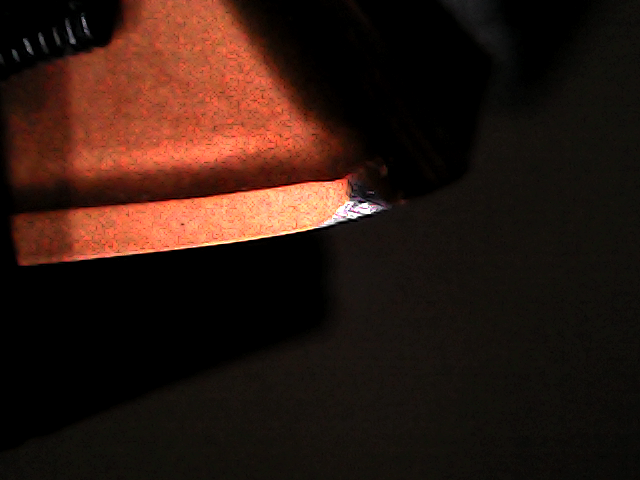
\includegraphics[width=\linewidth, keepaspectratio=true]{./fig/Vision/Dataset/automated_datasets/2_created_datasets/2_Spaghetti_dataset/rounded_gold_b_015_p_006_l_006-011_white_nb.png}
		\caption{Gold coloured insert.}
		\label{fig:impl:datasets:spaghetti:gold}
	\end{subfigure}
	\hspace*{\fill}
	\caption{Overview of different insert types.}
	\label{fig:impl:datasets:spaghetti:types}
\end{figure}

\paragraph{Set-up}

The set-up used is exactly the same as on the Birthday dataset where the camera is positioned as much to the top as possible as can be seen on Figure \ref{fig:impl:sd:setup:top}..
On Figure \ref{fig:impl:dataset:spaghetti:ledstrips} we can see the LED strips are a little bit twisted and are positioned very close to each other. This made the reflection better and should result in better outcome of the algorithm. The room in which the dataset was created was fully dark to have no other light sources influencing the reflections on the inserts.

\begin{figure}[hbtp]
\centering
	\hspace*{\fill}
	\begin{subfigure}{0.4\textwidth}
		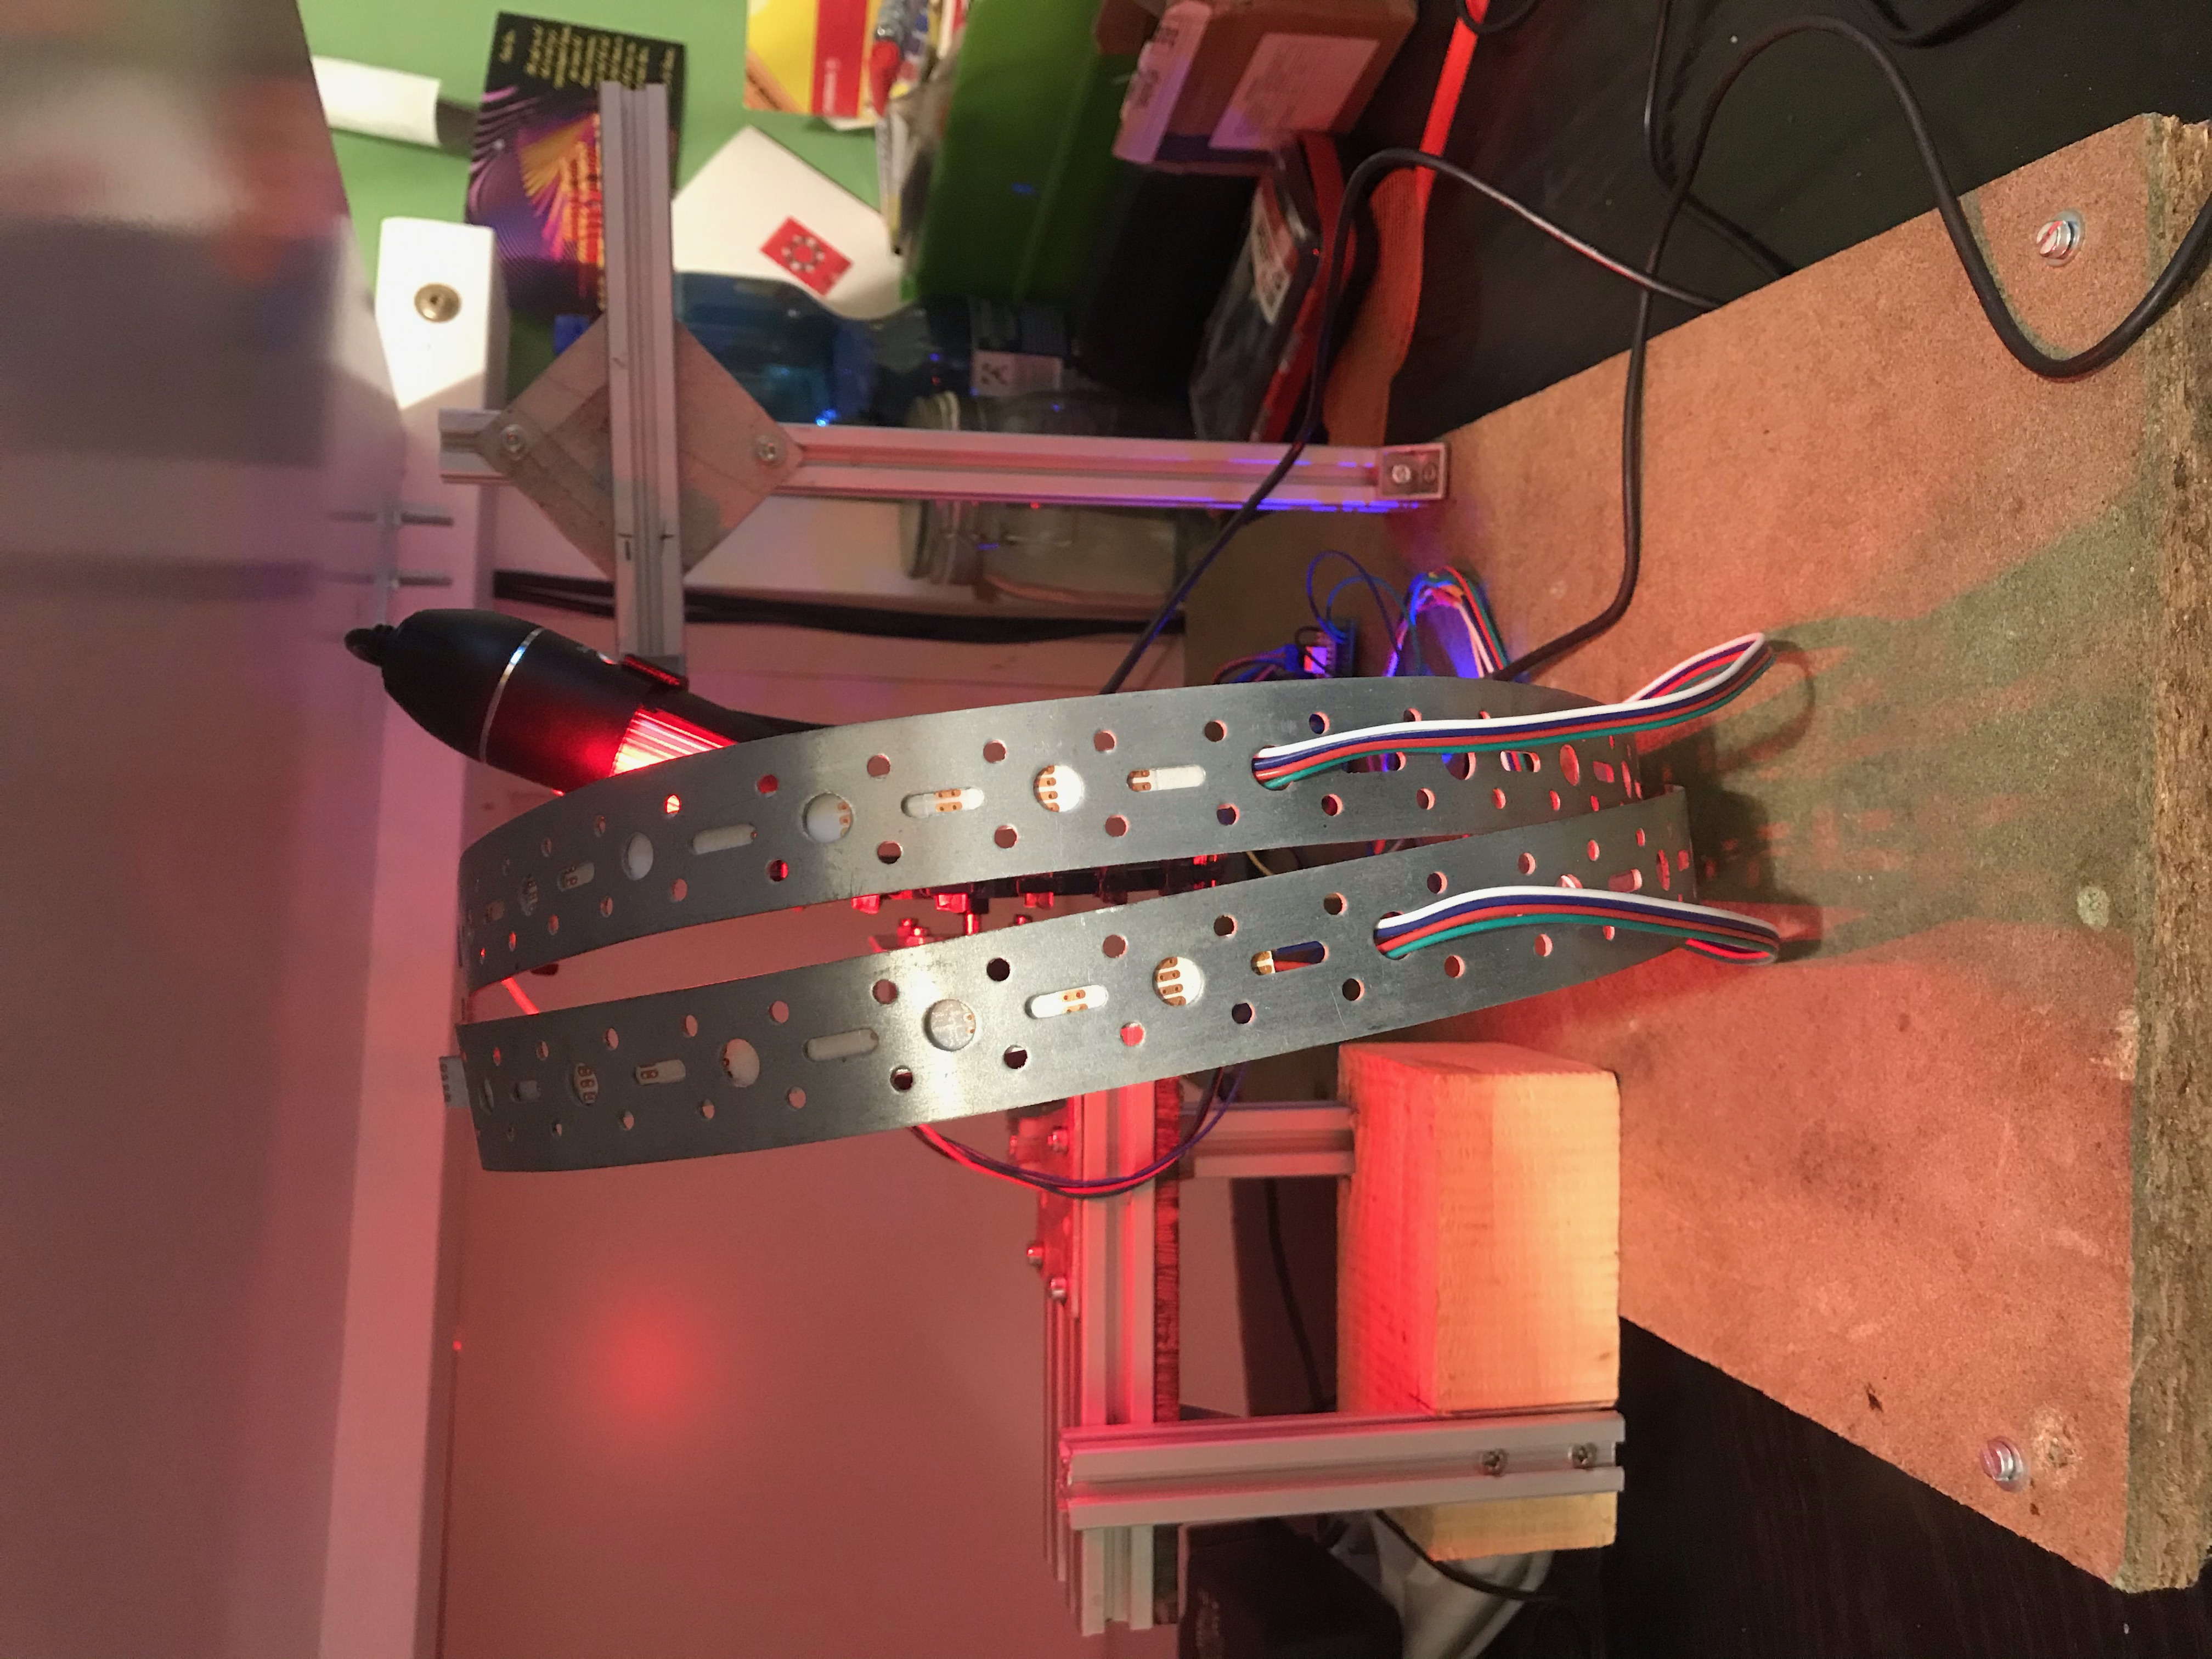
\includegraphics[width=\linewidth, keepaspectratio=true, angle=270]{./fig/Vision/Dataset/automated_datasets/2_created_datasets/2_Spaghetti_dataset/IMG_9295.jpeg}
		\caption{Setup with twisted LED strips.}
		\label{fig:impl:dataset:spaghetti:ledstrips}
	\end{subfigure}
	\hspace*{\fill}
	\begin{subfigure}{0.4\textwidth}
		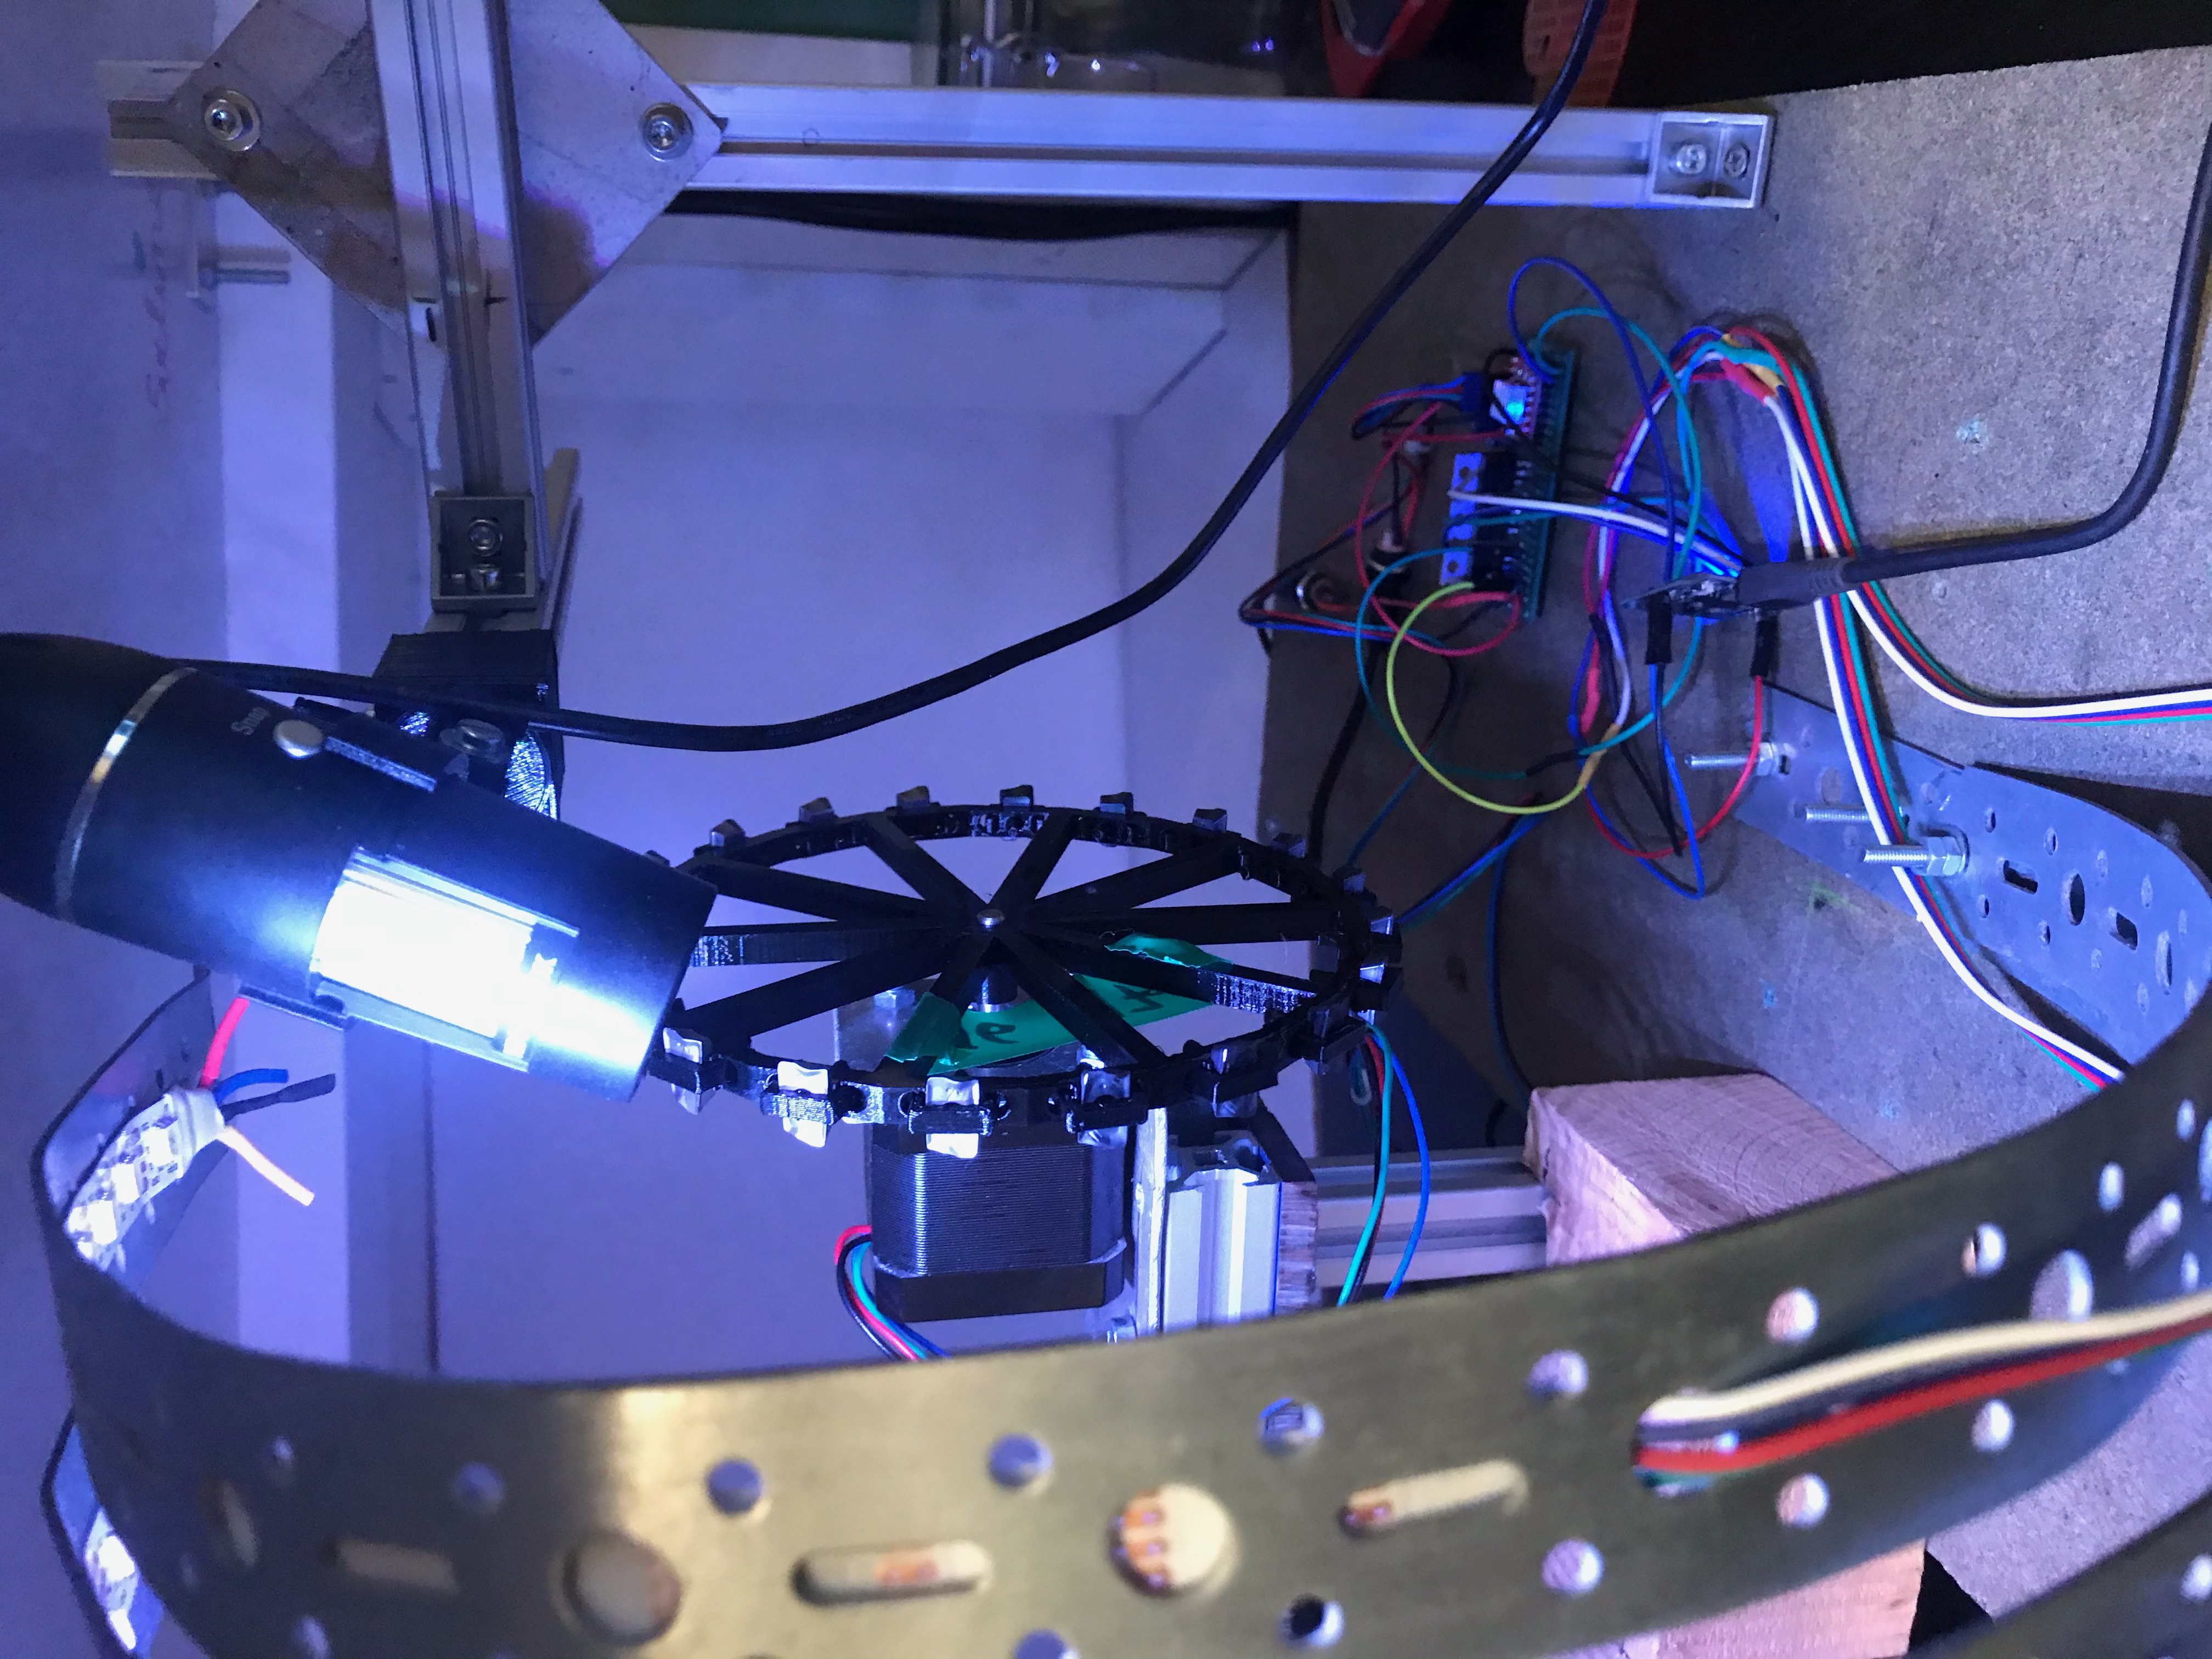
\includegraphics[width=\linewidth, keepaspectratio=true,angle=270]{./fig/Vision/Dataset/automated_datasets/2_created_datasets/2_Spaghetti_dataset/IMG_9296.jpeg}
		\caption{Test setup camera angle more to top.}
		\label{fig:impl:sd:setup:top}
	\end{subfigure}
	\hspace*{\fill}
	\caption{Overview of setup for the Spaghetti dataset.}
\end{figure}

\begin{figure}[hbtp]
\centering
	
\end{figure}



\paragraph{Results}

Figure \ref{fig:impl:datasets:spaghetti:result} shows two pictures of batch 3 insert 6. These where lit with red light in \ref{fig:impl:datasets:spaghetti:result:red} and white light in \ref{fig:impl:datasets:spaghetti:result:white}. Here is a nice wear shown and lighted. However if we zoom in to the picture the top part of the wear is not lighted that well. We can also see a white piece of the insert holder on the image which is providing some extra difficulties. There where also a few images not fully in focus in this dataset. The influence of these difficulties on the output of the neural network will be reviewed in section \ref{sec:results:spaghettivsshm}.

\begin{figure}[hbtp]
	\centering
	
	\hspace*{\fill}
	\begin{subfigure}{0.4\textwidth}
		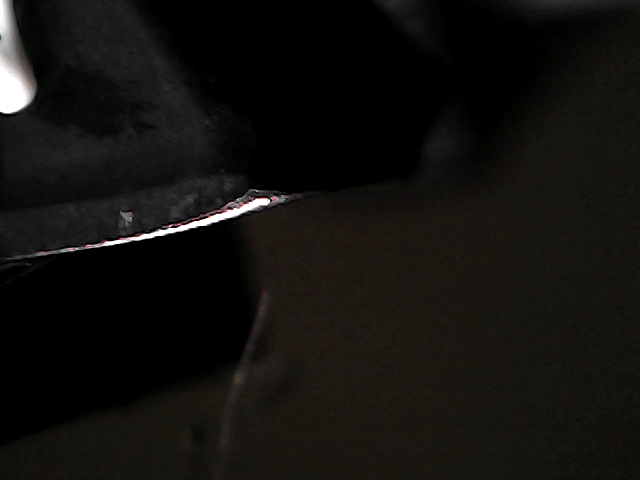
\includegraphics[width=\linewidth, keepaspectratio=true]{./fig/Vision/Dataset/automated_datasets/2_created_datasets/2_Spaghetti_dataset/b_003_p_006_l_006-011_white_nb.png}
		\caption{White light}
		\label{fig:impl:datasets:spaghetti:result:white}
	\end{subfigure}
	\hspace*{\fill}
	\begin{subfigure}{0.4\textwidth}
		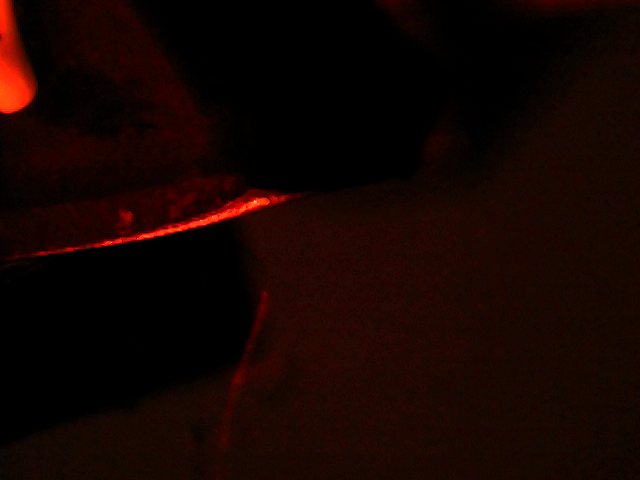
\includegraphics[width=\linewidth, keepaspectratio=true]{./fig/Vision/Dataset/automated_datasets/2_created_datasets/2_Spaghetti_dataset/b_003_p_006_l_006-011_red_nb.png}
		\caption{Red light}
		\label{fig:impl:datasets:spaghetti:result:red}
	\end{subfigure}
	\hspace*{\fill}
	\caption{Example images for red and white light for spaghetti dataset.}
	\label{fig:impl:datasets:spaghetti:result}
\end{figure}

\section{Vision algorithms}
\label{sec:impl:visionalgorithms}
	To test the camera setup, a classification model is made where inserts will be classified into three classes. The program overview is given in Figure \ref{fig:impl:va:prog:overview}. This section will be following the path on the figure starting with data organisation, going to model creation and ending with training and testing. The results obtained with these algorithms will be analysed in chapter \ref{chap:results}. 
	
	\begin{figure}[hbtp]
		\centering
		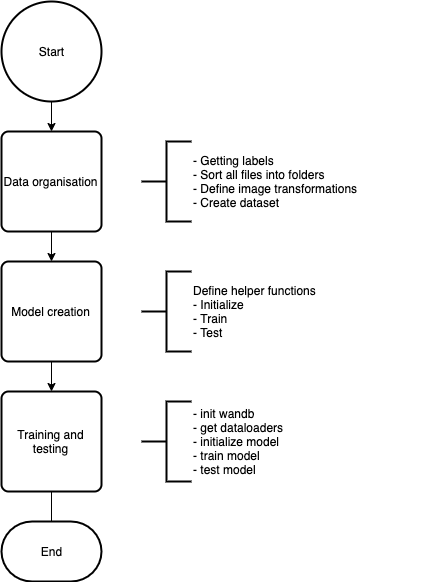
\includegraphics[width=0.6\textwidth]{fig/Vision/GoogleColab/Test_Camera_Setup/Program_sequention.png}
		\caption{Program sequention for testing different setups.}
		\label{fig:impl:va:prog:overview}
	\end{figure}
	
	\subsection{Data organisation}
	\label{sec:impl:visionalgorithms:dataorganisation}
		Before anything can be learned the data must be adjusted to provide a proper input to the model architectures. All these models require an input image of 224 by 224 pixels. First the labels are obtained from the labels file. Then the files are sorted into folders based on the class and function. After that the transformations on the images are defined to finally create a dataset. 
		
		\subsubsection{Getting labels}
		\label{sec:impl:va:do:labels}
			All labels where saved in an Excel file which was exported to the csv file type. The file was loaded using the pandas library for data analysis \citep{McKinney2015}. This file includes following columns for every insert:
			\begin{enumerate}
				\item Batch number (bn): provides the number of the batch, each batch consists of 10 inserts.
				\item Insert number (pn): The number of the insert in the batch in range 1 to 10.
				\item Bullet (b): Whether or not the side of insert has a "bullet" mark on it. An example was given in Figure \ref{fig:impl:va:do:bullet}
				\item Folder name: The name of the folder where the images of this insert are saved. This will contain the images for the two sides of the insert.
				\item Image name: Name of the image taken for the second handmade dataset. This field doesn't serve for the other datasets.
				\item Value: The measured wear value in $\mu$m.
			\end{enumerate}
			
		
	
			
		\subsubsection{Sorting images}
			The labels from \ref{sec:impl:va:do:labels} can now be used to divide images into the needed classes. For this task we will iterate over all possible images and decide to what set every image belongs and what class its value represents. 
			
			For every image there will be decided whether is goes in the training set, the test set or the validation set. The training set will hold 70\% of the images, the validation set will contain 20\% of the images. The remaining images will represent the test set which will be 10\% of all data.
			
			A random number will be generated between 1 and 3 which will represent one of these sets. According to this number the image belongs to a specific set. When a set is filled so it represents the amount specified by the percentage, the random number generator will only generate numbers 1 or 2 representing the remaining sets and so on.
			
			When the set is declared, the image must be divided into the three classes. This will be fulfilled by comparing the wear value of the image to two set limits. A lower limit of 130 $\mu$m and an upper limit of 230 $\mu$m. The division is given below:
			\begin{itemize}
				\item Class 1: Low wear between 0 $\mu$m and 130 $\mu$m
				\item Class 2: Medium wear between 130 $\mu$m and 230 $\mu$m
				\item Class 3: High wear between 230 $\mu$m and 1000 $\mu$m
			\end{itemize}		
			
			Now the set and class are known so the given image can be saved in a folder. The resulting folder structure is given in table \ref{tab:impl:visionalgorithms:folderstructure}.
			\begin{table}
			\centering
			\caption{Overview of folder structure.}
			\centering
			\begin{tabular}{c c c}
				Train 	& Test 	& Validation\\ \hline
				Low	& Low & Low \\ 
				Medium & Medium & Medium \\
				High	& High	& High\\
			\end{tabular}
			\label{tab:impl:visionalgorithms:folderstructure}
			\end{table}
			
		 Figure \ref{fig:impl:va:do:classdistr} shows the distribution of the classes for the first five batches in \ref{fig:impl:va:classdistr:1-5} and the distribution for all data in \ref{fig:impl:va:classdistr:all}. The class distribution should be 1/3 in the best case. The first graph shows a distribution which is close enough to this optimal distribution yet in the second graph we see the distribution is far from even which must be taken into account when analysing the results.

\begin{figure}[hbtp]
	\centering
	\begin{subfigure}{0.49\textwidth}
		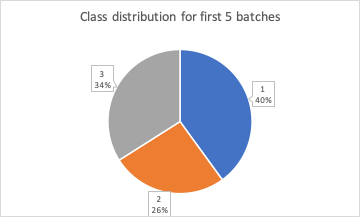
\includegraphics[width=\linewidth]{fig/Vision/GoogleColab/labels/class_distr_1-5.png}
		\caption{Class distribution for the inserts in batch 1 to 5.}
		\label{fig:impl:va:classdistr:1-5}
	\end{subfigure}
	\hspace*{\fill}
	\begin{subfigure}{0.49\textwidth}
		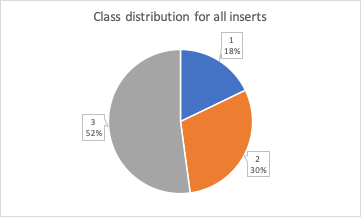
\includegraphics[width=\linewidth]{fig/Vision/GoogleColab/labels/class_distr_all.png}
		\caption{Class distribution for all inserts.}
		\label{fig:impl:va:classdistr:all}
	\end{subfigure}
	\caption{Class distributions for the inserts used for the algorithm training and testing}
	\label{fig:impl:va:do:classdistr}
\end{figure}

	\subsubsection{Image transformations}
	To provide more data from the images we already have, data augmentation is used where the images will be duplicated and transformed before being used as training and validation images. These transformations consist of a rotation between 0 and 4 degrees, a translation in both x and y direction of 0.2 times the width or height respectively and a shear of 0.1 also in both directions. After these transformation the images are rescaled to a 224 by 224 resolution since this is what the model architectures expects. The images are also normalized using the mean and standard deviation values from the Imagenet dataset \citep{imagenet_cvpr09}. This can be further optimized by calculating the mean and standard deviation of the full dataset ourselves but wasn't done for these tests.
	
	\subsubsection{Dataset creation}
	\label{sec:impl:do:dscreate}
	With all this done a dataset can finally be created by using PyTorch's ImageFolder function from the torchvision library. \citep{pytorch} 
	
	\subsection{Model creation}
		A few helper functions are defined for the model creation. One for initialisation of different model architectures. A second one to train the model and a third to test the model after training.
		
		\subsubsection{Model initialisation}
		\label{sec:impl:visionalgorithms:init}
			Every CNN architecture has an initialisation where the input and output sizes must be set. This input size will be 224 pixels by 224 pixels for all architectures used for the setup validation. The output size is a vector of size 3 which will store the probability for every class. Since this initialisation step is clustered in one function, more model architectures can be added easily. The following architectures are already implemented:
			
			\begin{itemize}
				\item Resnet18
				\item Alexnet
				\item VGG11\_bn
				\item Squeezenet
				\item Densenet
			\end{itemize}
			
			An initialisation for Inception v3 was also implemented as this was said to be well performing by \cite{Xu2019} in section \ref{sec:lit:va:un:other} but this did not seem to work. Due to time limitations the issue wasn't solved but will be solved in further researches on the exact value prediction of the tool wear.
			
		\subsubsection{Define training}
			The training of a CNN happens in two phases: a training phase and a validation phase. First the model will be trained with images gathered from one batch of images. This training phase will let some pictures of the batch go through the network and will adjust the weights of that network using back propagation. The back propagation can be done using different optimizers which will define how the weights are adjusted relative to the loss between the output of the model and the ground truth. As optimizer Stochastic Gradient Descent (SGD) is used. Cross entropy loss is used to calculate the loss between the output and the ground truth.
			
			When the training phase is finished, the training takes some images from the validation set to verify or validate the weights set by the training phase. This validation will check how the model reacts to pictures it wasn't trained on and therefore shows how the model works for general cases.
			
			The two described phases will be repeated for every epoch which will represent the duration of the training.
			
			During the whole process of training some values are logged to be able to check the training after it is done. For this purpose the training accuracy and loss are calculated and saved. The same values are stored for the validation phase. These values are logged using Weights and Biases (wandb) \citep{wandb} which will transform these logs into graphs and other useful data which can be seen in chapter \ref{chap:results}.
			
		\subsubsection{Define testing}
			In the data organisation section (\ref{sec:impl:visionalgorithms:dataorganisation}) a separate test set of images is created, this set will be used to evaluate the models performance. For this evaluation every picture from the test set will go through the model and the output will be compared to the ground truth. To log these tests, Weights and Biases is used as well where it saves some test pictures with their outputted class and the ground truth.
			
	\subsection{Training and testing}
		Finally the above functions will be used to actually train and test the model's performance. 
	For the training all data will be pushed to a GPU from Google Colaboratory.
		To perform the training a sweep is created on wandb which will generate a set of hyper parameters that will be passed on to the training function of the model. With these parameters a dataloader is created that will generate image batches using the created dataset from section \ref{sec:impl:do:dscreate}. These image batches will contain a specified amount of images defined by the batch size parameter. After this the model gets initialized, an optimizer is created as well as a loss criterion that will define the back propagation steps. Then the model is trained for a set amount of epochs hereafter the model is tested and the results are written to wandb.
		
		


